%\documentclass[12pt,draftcls,onecolumn]{IEEEtran}
\documentclass[journal]{IEEEtran}
%\IEEEoverridecommandlockouts  
%\overrideIEEEmargins     
\bibliographystyle{IEEEtran}
\pdfminorversion=4


\usepackage{cite}
%\usepackage{mathptmx}       % selects Times Roman as basic font
\usepackage{helvet}         % selects Helvetica as sans-serif font
\usepackage{courier}        % selects Courier as typewriter font
\usepackage{type1cm}        % activate if the above 3 fonts are
                            % not available on your system
%
\usepackage{makeidx}         % allows index generation
\usepackage{graphicx}        % standard LaTeX graphics tool
%                             % when including figure files
\usepackage{multicol}        % used for the two-column index
\usepackage{times}
\usepackage{xfrac}
\usepackage{caption}
\usepackage{subcaption}
%\usepackage{mathabx}
%\usepackage[thref]{ntheorem}
\usepackage{amsfonts}%
\usepackage{amssymb}%
\usepackage{amsthm}
\usepackage{mathrsfs}
\usepackage{url}
\usepackage{color}
%\usepackage{import}
\usepackage{graphicx,psfrag}
\usepackage{float}
\usepackage[cmex10]{amsmath}
\newtheorem{theorem}{Theorem}
\newtheorem{lemma}{Lemma}
\newtheorem*{remark}{Remark}
\newcommand{\jo}{(e^{-j\omega})}
\newcommand{\jok}{(e^{-j\omega_k})}
\newcommand{\jro}{(e^{-j\omega},\rho)}
\newcommand{\jrok}{(e^{-j\omega_k},\rho)}
%\renewcommand{\IEEEQED}{\IEEEQEDopen}
\renewcommand{\vec}[1]{\mathbf{#1}}
\newcommand{\hilight}[1]{\colorbox{yellow}{#1}}
%\DeclareRobustCommand*{\IEEEauthorrefmark}[1]{%
  %\raisebox{0pt}[0pt][0pt]{\textsuperscript{\footnotesize\ensuremath{#1}}}}

\title{\LARGE \bf A Robust Data-driven Controller Design Methodology for Particle Accelerator Power Converters}

%\iffalse
\author{Achille Nicoletti, Michele Martino and Alireza Karimi% <-this % stops a space

\thanks{Achille Nicoletti is with the Technology Department at
European Organization for Nuclear Research (CERN) and the Automatic Control Laboratory at
Ecole Polytechnique F\'{e}d\'{e}rale de Lausanne (EPFL) (email: \tt\small achille.nicoletti@cern.ch)}%
\thanks{Michele Martino is with the Technology Department at
European Organization for Nuclear Research (CERN) (email: \tt\small michele.martino@cern.ch)}%
\thanks{Alireza Karimi is with the Automatic Control Laboratory at
Ecole Polytechnique F\'{e}d\'{e}rale de Lausanne (EPFL) (email: \tt\small alireza.karimi@epfl.ch)}%
}
%\fi

\begin{document}

\maketitle
\thispagestyle{empty}
\pagestyle{empty}

\begin{abstract}
A new data-driven approach using the frequency response function (FRF) of a system is proposed for designing robust $H_{\infty}$ digital controllers for particle accelerators' power converters. This design method ensures that the dynamics of a system are captured and avoids the problem of unmodeled dynamics associated with parametric models. The $H_{\infty}$ robust performance condition can be represented by a set of convex constraints with respect to the parameters of a two-degree of freedom RST controller. This controller is robust with respect to the frequency-dependent uncertainties of the frequency response function. Moreover, constraints will be imposed in order to simultaneously ensure the desired stability margins and the controller stability. A convex optimization algorithm is then implemented to obtain the controller parameters. The effectiveness of the method is illustrated by designing the controller for the Q-STRIP magnet power converter of the PS Booster accelerator upgrade project at CERN. Experimental validation in the time domain is also presented. 
\end{abstract}

\begin{IEEEkeywords}
Convex optimization, data-driven control, H-infinity, power converter control, robust control, RST %uncertainty, Smith predictor, MIMO time delay. 
\end{IEEEkeywords}


\section{Introduction}
\IEEEPARstart{M}{any} of today's  complex systems possess a multitude of uncertainties, and obtaining an accurate parametric model for such systems can be both laborious and impractical for controller synthesis. In industrial schemes, the dynamics of plants are typically approximated by low-order models, since the controller synthesis is easier to implement for lower order processes. However, this approximation can impede the  performance of a controller, since low-order models are subject to model uncertainty. A survey on the differences associated with model-based control and data-driven control has been addressed in \cite{HW13} and \cite{BCE12}; the authors assert that model-based control methods are inherently less robust due to the unmodeled dynamics of a process, and that these controllers are unsafe for practical applications. With the data-driven control scheme, the parametric uncertainties and the unmodeled dynamics are irrelevant and the only source of uncertainty is the measurement noise. 

Data-driven controllers can be synthesized either on-line or off-line; the on-line methods such as the classical direct adaptive control (MRAC) \cite{LLMK11}, model-free adaptive control (MFAC) \cite{HJ13}, and the unfalsified control (UC) \cite{ST97} methodologies design controllers using time-domain data. Iterative feedback tuning (IFT) \cite{Hja02}, correlation-based tuning (CBT) \cite{KMB02a}, virtual reference feedback tuning (VRFT) \cite{CLS02}, non-iterative data-driven model reference control \cite{KVB07} methodologies are all off-line time-domain data-driven methods.  The widely used PID controller is usually tuned based on a set of time-domain or frequency-domain data. 

Data-driven control methods using frequency-domain data are design schemes that continue to spark the interest of many researchers. The frequency-domain approach offers many advantages compared to time-domain methods :
\begin{itemize}
\item Without knowledge of the transfer function, the dynamics of a system can be captured experimentally through the frequency response.
\item Relative and absolute stability of a closed-loop system can be determined with the knowledge of the open-loop frequency response.
\item Noise disturbance generated in the system can be easily determined using frequency analysis.
\item System uncertainties can be modeled at discrete frequency points (which reduces the conservatism associated with uncertainty modeling). 
\end{itemize}
The authors in \cite{HDAV10} use the frequency response data of a stable system to design an optimal controller through a symmetric root locus technique. A robust frequency-domain control design method has been established in \cite{KNND13b}; this method, however, requires a solution to a non-linear optimization problem. A frequency-domain loop-shaping approach to design fixed-structure controllers is presented in \cite{KNND13c}. In this method, a convex optimization problem can be formulated if a linearly parameterized controller is considered; however, in this method, the closed-loop stability is not guaranteed and should be verified a posteriori. Robust controller design methods belonging to the $\mathcal{H}_{\infty}$ control framework minimizes the $\mathcal{H}_{\infty}$ norm of a weighted closed-loop sensitivity functions. In \cite{DWS09} a frequency-response method is proposed based on the $Q$-parametrization to guarantee the $\mathcal{H}_{\infty}$ performance for fixed-structure controllers. In \cite{KG10}, a frequency domain approach is realized where a convex optimization algorithm is formulated by considering a convex approximation of the $\mathcal{H}_{\infty}$ criterion. In order to obtain convexity, however, the controller is chosen to be linearly parameterized, i.e. the denominator of the controller are fixed. This limits the number of degrees of freedom of the controller, and thus impedes the controller performance. A frequency-domain approach for computing low-order multivariable linearly parameterized controllers is presented in \cite{SOW10}. The $\mathcal{H}_{\infty}$ constraints are convexified around an initial stabilizing controller. An iterative algorithm is used that converges to a local optimal solution of the non-convex problem. The method in \cite{KG10} is extended to data-driven gain-scheduled controller design in \cite{KE13a} and multivariable decoupling controller design in \cite{GKL10b}. A public domain toolbox for Matlab is also available \cite{Kar13}. A similar approach is proposed in  \cite{HAB13}, where a convex-concave approximation of the $\mathcal{H}_{\infty}$ constraints based on an initial stabilizing controller is used. The extension of this method to design multivariable PID controllers for stable systems is presented in \cite{BHA16}. This method uses the same convex approximation as in  \cite{SOW10} but is limited to stable systems and PID structure. The design of controllers that are not linear in parameters (e.g. represented by rational transfer functions) using frequency domain data are studied in \cite{KNZ16}. The necessary and sufficient conditions for the existence of such controllers are developed. This method needs no initial stabilizing controller and converges to the optimal  $\mathcal{H}_{\infty}$ performance when the order of the controller goes to infinity.

%\iffalse
%Generally, it is desired to formulate a convex optimization problem for controller synthesis, since convex problems are computationally tractable. A frequency domain approach in designing the $RST$ controllers has been discussed in \cite{MRS11}, where a convex optimization problem is formulated by bounding a specific sensitivity function and specifying a desired characteristic polynomial. Robust stability, however, is not trivially achieved, since the characteristic polynomial incorporates an observer polynomial which usually needs to be tuned iteratively. With $\mathcal{H}_{\infty}$ control techniques, it is possible to eliminate the necessity of using observer polynomials for achieving proper robustness margins. Robust controller design methods belonging to the $\mathcal{H}_{\infty}$ control framework minimizes the $\mathcal{H}_{\infty}$ norm of a weighted closed-loop sensitivity function. In \cite{GKL11}, a frequency domain approach is realized where a convex optimization algorithm is formulated by considering a convex approximation of the $\mathcal{H}_{\infty}$ criterion. With this method, suitable robustness margins are attainable; however, in order to preserve convexity, this method requires one of the controller terms ($R$) to be fixed a priori\footnote{Note that the variable names for $R$ and $S$ are interchanged in \cite{GKL11}}. This limits the number of degrees of freedom of the controller, and thus impedes the controller performance. 


The $RST$ controller structure is an effective discrete-time two-degree of freedom (2DOF) polynomial controller where the tracking and regulation characteristics of a closed-loop system can be formulated independently \cite{LZ06}. 
The $RST$ controller design methodology is usually based on the pole placement technique and uses the dynamic model of the physical system. In \cite{GKL11}, the data-driven frequency-domain approach of \cite{KG10} is extended to $RST$ controller design. However, in order to preserve convexity, this method requires one of the controller terms to be fixed a priori. This problem is fixed in \cite{NEK15}, where an $RST$ controller is designed in the $\mathcal{H}_{\infty}$ framework by formulating a convex optimization problem in a data-driven setting. The necessary and sufficient conditions for the existence of $RST$ controllers that satisfy the  $\mathcal{H}_{\infty}$ constraint only on one sensitivity function are also developed. 


The proposed method in this paper is an extension of \cite{NEK15}, where the necessary and sufficient conditions that ensures the $\mathcal{H}_{\infty}$ performance for multiple weighted sensitivity functions is presented. Moreover, the frequency-dependent uncertainties originated from the measurement noise are taken into consideration for robust performance specifications. Additionally, since the parameters of the controller's denominator are the optimization variables, this method can lead to unstable controllers. Therefore, a sufficient condition is presented to ensure that the controller remains stable. The proposed method is then used to design a robust $RST$ controller for power converters in particle accelerators at CERN. The designed controller is implemented in the power converters to control their output current with extremely high precision. The main advantage of the proposed method for this application is to guarantee the robustness margins, high bandwidth and small tracking error by a data-driven convex optimization based approach that does not require the manual tuning of the classical pole-placement model-based approach.

The paper is organized as follows.
The class of models, controllers and control objectives are defined in section (\ref{sec:2}). Section (\ref{sec:3}) discusses the control design methodology and stability conditions of the proposed method for the $RST$ controller structure. Convex conditions are formulated based on the $\mathcal{H}_{\infty}$ criterion. Section (\ref{sec:4}) discusses the framework of the power converter control system and its functionality at CERN. Section (\ref{sec:5}) is dedicated to a case study where the effectiveness of the method is demonstrated by applying the proposed design scheme to a power converter control system for a specific accelerator requirement. Finally, the concluding remarks are given in section (\ref{sec:6}).

%\textbf{Notation}: In order to avoid the risk of any confusion, the notation for the symbols employed in this paper will be defined here.
%\begin{align*}
%\mathbb{R}/ \mathbb{R}^+ &: \ \mbox{the set of all real numbers/positive real numbers.} \\
%\mathbb{Z} &: \ \mbox{the set of non-negative integers.} \\
%\mathcal{R}e\{X \} &: \ \mbox{the real part of a complex variable }X. \\
%\mathcal{I}m\{X \} &: \ \mbox{the imaginary part of a complex variable }X. \\
%a^{\top} &: \ \mbox{the transpose of the vector }a. \\
%z &: \ \parbox[t]{18em}{complex frequency variable used to represent discrete-time systems.} \\
%s &: \ \parbox[t]{18em}{complex frequency variable used to represent continuous-time systems.}
%\end{align*} 
%\section{Notation and Preliminaries}
%Due to the nature of the equations asserted in this paper, it will be convenient express certain equations in a compact manner. A cascade of $q$ frequency response functions $A_1(e^{-j\omega})A_2(e^{-j\omega}) \cdots A_q(e^{-j\omega})$ will be denoted as $[A_1A_2 \cdots A_q](e^{-j\omega})$. 


\section{Problem Formulation}
\label{sec:2}
\subsection{Preliminaries}
Let $u[k]$ and $y[k]$ represent the input and output signals of a causal discrete-time system, respectively, where $k$ is a discrete-time instant and $T_s$ is the sampling period. Suppose that these signals are noise-free and have zero initial and final conditions (i.e., $u[k] = y[k] = 0$ for $k \leq 0$ and $k > K_s$). Then, the frequency response function (FRF) of the system can be represented as 
\begin{equation}
G(e^{-j\omega}) = Y(e^{-j\omega}) U^{-1}(e^{-j\omega})
\end{equation}
where
\begin{align}
U(e^{-j\omega}) &= \frac{1}{\sqrt{K_s}} \sum_{k=0}^{K_s} u[k]e^{-j \omega T_s k} \label{eq:U_period}\\
Y(e^{-j\omega}) &= \frac{1}{\sqrt{K_s}} \sum_{k=0}^{K_s} y[k]e^{-j \omega T_s k}
\end{align} 
are the periodograms of the input and output signals and $\omega \in [-\pi/T_s, \pi/T_s]$. Note that due to the symmetry of the periodograms, it is sufficient to consider $\omega \in [0, \pi/T_s]$ for practical applications. Under these assumptions, it is evident that from a set of sampled time-domain data, one is able to obtain a continuous FRF.  If the data is noisy, then $G(e^{-j\omega})$ is characterized as the Empirical Transfer Function Estimate (ETFE) and is asymptotically unbiased \cite{Lju99}. For such systems, a multiplicative uncertainty can be considered to ensure robustness in the presence of noise perturbations. 

Let the set $\mathscr{P}$ represent the family of all stable, proper, real-rational discrete-time transfer functions with no pole on the unit circle. It is imperative to note that $\mathscr{P}$ is closed under multiplication and addition; in other words, if $P_1(z^{-1}),P_2(z^{-1}) \in \mathscr{P}$, then 
\begin{equation}
\{ P_1(z^{-1})+P_2(z^{-1}),P_1(z^{-1})P_2(z^{-1})\} \in \mathscr{P}
\end{equation}
Suppose that a single-input-single-output (SISO) feedback control system structure is used where the plant is represented as $G(z^{-1}) = N(z^{-1})M^{-1}(z^{-1})$ such that $\{N(z^{-1}),M(z^{-1})\} \in \mathscr{P}$. As asserted in \cite{ZD98} and \cite{DFT92}, if $\{N(z^{-1}), M(z^{-1})\} \in \mathscr{P}$, then $G(z^{-1}) = N(z^{-1})M^{-1}(z^{-1})$ is called a \textit{coprime factorization} of $G(z^{-1})$ over $\mathscr{P}$.

\subsection{Class of models}
Let the FRF of such a factorized discrete-time SISO plant be defined as follows:
\begin{equation}\label{eq:setpmimo}
G\jo = N\jo M^{-1}\jo, \qquad \forall \omega \in \Omega
\end{equation}
where $\Omega \in [0,\pi/T_s]$. $N\jo$ and $M\jo$ must be FRF's of bounded analytic functions outside the unit circle; for a stable plant, a trivial choice is $N\jo=G\jo$ and $M\jo=1$. A discussion on how to formulate $N\jo$ and $M\jo$ for unstable processes can be found in \cite{KNZ16}. In general, a set $\mathcal{G}$ can be formulated to represent a plant model containing $p$ FRF models:
\begin{equation}
\mathcal{G} = \{G_l\jo; \quad l=1,\ldots,p; \quad \forall \omega \in \Omega\}
\end{equation} 
These FRF's can be determined by considering the frequency response of a parametric model or from a set of input/output data. For simplicity, one model from the set $\mathcal{G}$ will be considered, and the subscript $l$ will be omitted. However, in general, the design procedures outlined in this paper can be applied to the multi-model case. %In fact, in Section (\ref{sec:4}), a multi-model case will be investigated for the controller synthesis of the power converter control system. 

\subsection{Frequency-domain uncertainty} \label{sec:freq_uncertain}
Suppose that the uncertainty associated with a given FRF is described by an additive uncertainty:
\begin{equation}
\begin{aligned} \label{eq:frf_uncertainty}
\hat{N}(e^{-j\omega}) &= N(e^{-j\omega}) + |W_n(e^{-j\omega})| \delta_n e^{j\theta_n} \\
\hat{M}(e^{-j\omega}) &= M(e^{-j\omega}) + |W_m(e^{-j\omega})| \delta_m e^{j\theta_m}
\end{aligned}
\end{equation}
where $|\delta_n| \leq 1$, $|\delta_m| \leq 1$; $\{ \theta_n,\theta_m\} \in [0,2\pi]$; $W_n$ and $W_m$ are the uncertainty weighting filters which can be determined from the covariance of the estimates for a given confidence interval.  As previously stated, $N\jo = G\jo$ and $M\jo = 1$ can be selected for stable systems. Therefore, given the periodogram of $G$, the estimates of the real and the imaginary part of $N\jo$ can be formulated; these estimates are asymptotically uncorrelated and normally distributed with a variance of $\Phi_v(\omega)/2|U\jo|^2$, where $\Phi_v(\omega)$ is the spectrum of the disturbance $v[k]$ at the output of the plant (\cite{Lju99}). The additive uncertainty can be described in the complex plane with a disk centered at $N\jo$ having a radius of $|W_n\jo|$. The uncertainty is characterized by the Rayleigh distribution and can be determined for any probability level. For example, if it is desired to construct an uncertainty disk such that the true frequency response lies within the disk with a probability level of $0.95$, then the radius of this disk will be
\begin{equation} \label{eq:uncertainty_radius}
|W_n\jo| = \sqrt{\frac{5.99 \Phi_v(\omega)}{2|U\jo|^2}}
\end{equation}
The output noise spectrum can be estimated as
\begin{equation} \label{eq:noise_spectrum}
\Phi_v(\omega) = \Phi_y(\omega) - \frac{|\Phi_{uy}(\omega)|^2}{\Phi_u(\omega)}
\end{equation}
where $\Phi_u(\omega)$ is the input spectrum, $\Phi_y(\omega)$ is the output spectrum, and $\Phi_{uy}(\omega)$ is the cross-spectral density of the input and output channels. 

\subsection{Class of controllers}
\begin{figure}
\centering
\resizebox{1\columnwidth}{!}{\input{rst.eps_tex}}
\caption{$RST$ controller structure}
\label{fig:rst}
\end{figure}
The controller structure that will be considered will be of the $RST$-type. The $RST$ controller is a two-degree of freedom controller which can be used to synthesize the tracking and regulation requirements independently from each other \cite{LZ06}. The general structure of this controller is shown in Fig.~\ref{fig:rst}. Each controller is realized as a polynomial function as follows:
\begin{alignat}{2}
R(z^{-1},\rho) &= r_0 + r_1z^{-1} + \cdots + r_{n_r}z^{-n_r} \label{eq:Rc}\\
S(z^{-1},\rho) &= 1 + s_1z^{-1} + \cdots + s_{n_s}z^{-n_s} \label{eq:Sc}\\
T(z^{-1},\rho) &= t_0 + t_1z^{-1} + \cdots + t_{n_t}z^{-n_t} \label{eq:Tc}
\end{alignat}
where $\{n_s,n_r,n_t\}$ are the orders of the polynomials $R,S$ and $T$, respectively. These controllers can also be represented in a linear regression form as 
\begin{align}
R(z^{-1},\rho)&=\rho_R^\top \phi_{n_r}(z^{-1})= [r_0,r_1,\ldots,r_{n_r}]\phi_{n_r}(z^{-1}); \nonumber \\
S(z^{-1},\rho)&=\rho_S^\top \phi_{n_s}(z^{-1})= [1,s_1,\ldots,s_{n_s}]\phi_{n_s}(z^{-1}); \nonumber \\
T(z^{-1},\rho)&=\rho_T^\top \phi_{n_t}(z^{-1})= [t_0,t_1,\ldots,t_{n_t}]\phi_{n_t}(z^{-1}); \nonumber
\end{align}
where
\begin{align}
\rho^\top &=[\rho_R^\top, \rho_S^\top, \rho_T^\top] \nonumber \\
\phi_x^\top(z^{-1}) &= [1,z^{-1},\ldots,z^{-x}] \nonumber
\end{align}
%The purpose of parameterizing the controllers in this manner will become apparent in subsequent sections. 
where $x \in \{n_r,n_s,n_t \}$.
 
Based on the internal model principle, the controller may contain the disturbance model to achieve a zero steady-state error. Therefore, the polynomials may be pre-multiplied with any arbitrary function that actualizes the desired action. For example, if it is desired to reject a step disturbance at the output, then $S(z^{-1},\rho)$ can be pre-multiplied with $(1-z^{-1})$ (which represents the integral action of the controller). For sinusoidal disturbances at specific frequencies, the polynomials can be pre-multiplied with the function
\begin{equation*}
\theta (z^{-1}) = 1-2z^{-1} \cos(\omega_z T_s) + z^{-2}
\end{equation*}  
where $\omega_z$ is the frequency in $rad/s$ at which the disturbance occurs. %Suppose that there is noise $v$ at a frequency $\omega_z$, and is it desired to attenuate the effects caused by this disturbance (note that (\ref{eq:V}) represents the sensitivity function of interest for this disturbance). Then the $R$ polynomial can be pre-multiplied with $\theta (z^{-1})$ to achieve the desired noise attenuation at the output. In general, any of the $RST$ polynomials can be pre-multiplied with any polynomial that performs the desired action.
%The purpose of parameterizing the controllers in this manner will become apparent in subsequent sections.
%For notation purposes, the dependency on the discrete-time frequency variable $z^{-1}$ will be omitted, and the dependency on the controller parameter $\rho$ will remain. 


\subsection{Sensitivity Functions}
\label{sec:23}
Since the design techniques introduced in this paper belong to the $\mathcal{H}_{\infty}$ framework, it is  appropriate to consider the various sensitivity functions associated with the $RST$ controller structure. Some sensitivity functions for this process can be asserted as follows:
\begin{align}
\mathcal{S}_1(z^{-1},\rho)&= \frac{y}{d_o} = \frac{M(z^{-1})S(z^{-1},\rho)}{\psi(z^{-1},\rho)}  \label{eq:S0}\\
\mathcal{S}_2(z^{-1},\rho)&= \frac{y}{r} =\frac{N(z^{-1})T(z^{-1},\rho)}{\psi(z^{-1},\rho)} \label{eq:T} \\
\mathcal{S}_3(z^{-1},\rho)&= \frac{r-y}{r} =\frac{\psi(z^{-1},\rho)-N(z^{-1})T(z^{-1},\rho)}{\psi(z^{-1},\rho)} 
\end{align}
where $\psi(z^{-1},\rho) = N(z^{-1})R(z^{-1},\rho)+M(z^{-1})S(z^{-1},\rho)$, $y$ is the system output, $r$ is the reference input, and $d_o$ is the output disturbance. For notation purposes, the dependency in $z^{-1}$ will be omitted, and will only be reiterated when deemed necessary. Note that all of the sensitivity functions are stable if the zeros of $\psi(\rho)$ lie within the unit circle. The sensitivity functions defined above (and all other sensitivity functions of interest) all contain the same transfer function  $\psi(\rho)$. Therefore, a general construction of the sensitivity function can be expressed as $\mathcal{S}_q(\rho) = \Delta_q(\rho)/ \psi(\rho)$, where $\Delta_q(\rho)$ is a linear function of $R$, $S$ and/or $T$. The subscript $q \in \{ 1,2,\ldots,c\}$ denotes the $q$-th sensitivity of interest and $c$ is the total number of sensitivity functions. 




\section{$\mathcal{H}_{\infty}$ Performance via Convex Optimization}
\label{sec:3}
\subsection{General Design Specifications}
\label{sec:general}
In the general $\mathcal{H}_\infty$ control problem, the objective is to find the controller parameters vector $\rho$ such that
\begin{equation} \label{eq:true_hinf}
\sup_{\omega \in \Omega} |H_q(e^{-j\omega},\rho)| < \gamma
\end{equation}
where $\gamma \in \mathbb{R}^+$, $H_q(e^{-j\omega},\rho) = W_q(e^{-j\omega}) \mathcal{S}_q(e^{-j\omega},\rho)$ and $W_q$ is the FRF of a stable weighting filter such that $H_q(e^{-j\omega},\rho)$ has a bounded infinity norm. For notation purposes, the dependency in $e^{-j\omega}$ will be omitted, and will only be reiterated when deemed necessary. The condition in (\ref{eq:true_hinf}) can also be expressed as follows:
\begin{equation} \label{eq:circle}
\gamma^{-1}|W_q \Delta_q(\rho)| < |\psi(\rho)| ; \quad \forall \omega \in \Omega
\end{equation}

It is desired to minimize the upper bound $\gamma$ such that the $\mathcal{H}_{\infty}$ performance condition is satisfied. 
Therefore, the following optimization problem can be considered:
\begin{equation} \label{eq:min1}
\begin{aligned}
& \underset{\rho}{\text{minimize}}
& & \gamma  \\
& \text{subject to:} & & \gamma^{-1} |W_q\Delta_q(\rho)| < |\psi(\rho)|  \\ 
& & & \forall \omega \in \Omega \quad ; \quad  q \in \mathcal{Q} \subset \{1, 2, \ldots, c\}
\end{aligned}
\end{equation}
Notice that (\ref{eq:min1}) is a non-convex optimization problem.


\begin{figure}
\hspace*{1cm}
\resizebox{0.9\columnwidth}{!}{\input{nxmy2_rad_diff_2.eps_tex}}
\caption{The graphical interpretation of $\mathcal{H}_{\infty}$ constraints in the complex plane}
\label{fig:circle}
\end{figure}

Consider a circle in the complex plane at a specific frequency in $\Omega$ which is centered at $\psi(\rho)$ and has radius $\gamma^{-1}|W_q\Delta_q(\rho)|$. The constraint in (\ref{eq:circle}) ensures that for any frequency point in $\Omega$, the circle associated with this frequency point will not encircle the origin. Fig.~\ref{fig:circle} displays the graphical interpretation of this condition. This geometrical construction will be used to prove the following Lemma:

\begin{lemma}   \label{lem2}
Suppose that $$H_q(\rho,e^{-j\omega})={W_q\jo \Delta_q(\rho,e^{-j\omega})} \psi^{-1}(\rho,e^{-j\omega})$$ is the frequency response of a bounded analytic function outside the unit circle. Then, the following constraint is met
\begin{equation} \label{eq4}
\sup_{\omega \in \Omega}  |H_q(\rho,e^{-j\omega})| < \gamma
\end{equation}
if and only if there exists a finite-impulse-response (FIR) function $F(z^{-1})$ that satisfies
$$
\Re\{\psi(\rho)F(e^{-j\omega})\}>\gamma ^{-1}|W_q\Delta_q(\rho)F(e^{-j\omega})|,  \qquad \forall \omega \in \Omega 
$$
\end{lemma}

{\it Proof :} 
The basic idea is similar to that of  the proof of Theorem~1 in \cite{RM94}. It is clear that (\ref{eq4}) is satisfied if and only if the disk of radius $ \gamma ^{-1}|W_q\Delta_q(\rho)|$ centered at $\psi(\rho)$ does not include the origin for all $\omega \in \Omega$, i.e. $|\psi(\rho)|>\gamma ^{-1}|W_q\Delta_q(\rho)|$. This is equivalent to the existence of a line passing through origin that does not intersect the disk. Therefore, at every given frequency, $\omega$, there exists a complex number $f(e^{-j\omega})$ that can rotate the disk such that it lays inside the right hand side of the imaginary axis. Hence, we have 
\begin{equation}
\label{eq:lem_eq1}
\begin{split}
\Re \left\{ \left[ \psi(\rho) - \gamma ^{-1}|W_q\Delta_q(\rho)|e^{j\theta} \right] f(e^{-j\omega}) \right\}>0 \\
\forall \omega \in \Omega, \forall \theta \in [0 \, , \, 2 \pi [
\end{split}
\end{equation}
where $\Re \{ \cdot \}$ denotes the real part of a complex variable. Since $f(e^{-j\omega}) = |f(e^{-j\omega})|e^{j\theta_f}$, then the above condition can be expressed as
\begin{equation}
\label{eq:lem_eq2}
\begin{split}
\Re\{  \psi(\rho)f(e^{-j\omega}) \}> \gamma ^{-1}|W_q\Delta_q(\rho)f(e^{-j\omega})|\cos(\theta + \theta_f) \\
\forall \omega \in \Omega, \forall \theta \in [0 \, , \, 2 \pi [
\end{split}
\end{equation}
However, (\ref{eq:lem_eq2}) is satisfied if and only if:
\begin{equation}
\label{eq18}
\begin{split}
\Re\{  \psi(\rho)f(e^{-j\omega}) \}> \gamma ^{-1}|W_q\Delta_q(\rho)f(e^{-j\omega})| \\
\forall \omega \in \Omega
\end{split}
\end{equation}
In \cite{RM94}, it is shown that, $f(e^{-j\omega})$ can be approximated arbitrarily well by the frequency response of a stable transfer function or FIR function $F(z^{-1})$ if and only if 
\begin{equation}
Z=\left( \psi(\rho) - \gamma_0 ^{-1}|W_q\Delta_q(\rho)|e^{j\theta} \right)^{-1}
\end{equation}
is analytic in the right half plane for all $\gamma_0>\gamma$ and all $\theta \in [0 \, , \, 2 \pi [$. However, $\psi^{-1}(\rho)$ is stable because of the stability of $H_q(\rho)$. On the other hand, by decreasing $\gamma_0$ from infinity to $\gamma$, the poles of $Z$ move continuously with $\gamma_0$. Therefore, $Z$ is not analytic in the right half plane if and only if $Z^{-1}(e^{-j\omega})=0$ for a given frequency, which is not the case because the origin is not in the interior of the circle $\gamma_0 ^{-1}|W_q\Delta_q(\rho)|e^{j\theta}$.  
{\hfill \ensuremath{\blacksquare}}

The set of all controllers that meet the performance condition defined by the weighted norm of sensitivity functions is asserted in the following theorem.

\begin{theorem}  \label{Th1}
Given the frequency response function $G\jo = N\jo M^{-1}\jo$ and the frequency response of a weighting filter $W_q\jo$, then the following statements are equivalent for a given $q \in \mathcal{Q}$: 

{\bf (a)} There exists an $RST$ controller that stabilizes $G$ and 

	\begin{equation}
	\label{state_a_single}
	\begin{aligned}
	\sup_{\omega \in \Omega}  | {W_q \mathcal{S}_q(\rho)} | < \gamma 
	\end{aligned}
	\end{equation}
	
    %\begin{equation}
	%\label{state_a}
	%\sup_{\omega \in \Omega}  | {W_0 (1+GK)^{-1}} | < \gamma
	%\end{equation}


{\bf (b)} There exists an $RST$ controller such that
\begin{equation} \label{state_b_single}
\begin{aligned}
\Re\{\psi(\rho)\}  >\gamma ^{-1}|W_q\Delta_q(\rho)|\quad \forall \omega \in \Omega
 \end{aligned} 
\end{equation}
\end{theorem}
{\it Proof :} ({\bf b} $\Rightarrow$ {\bf a}) 
$\psi(\rho)$ is analytic outside the unit circle and its real part is positive for all $\omega \in \Omega$. Therefore, $\psi(\rho)$ will not encircle the origin when $\omega$ travels along the Nyquist contour, and its inverse is stable. This implies that $R(\rho)$ and $S(\rho)$ stabilizes $G$. On the other hand, we have
\begin{equation}  \nonumber
\begin{aligned}
|\psi(\rho)| \geq \Re\{\psi(\rho)\} \quad 
\forall \omega \in \Omega
\end{aligned}
\end{equation}
which leads to
\begin{equation} \label{eq:the_1_single_2}
\begin{aligned}
|W_q\Delta_q(\rho)| < \gamma |\psi(\rho)| \quad \forall \omega \in \Omega
 \end{aligned}
\end{equation}
Therefore, (\ref{eq:the_1_single_2}) leads to (\ref{state_a_single}) in Statement ({\bf a}).  

({\bf a} $\Rightarrow$ {\bf b}) Assume that $R(\rho_0)$,  $S(\rho_0)$, and/or\footnote{The inclusion of $T(\rho_0)$ depends on which sensitivity function $\mathcal{S}_q^0(\rho)$ is being considered} $T(\rho_0)$ satisfies Statement ({\bf a}) but not Statement ({\bf b}). Then, according to Lemma 1, there exists a FIR function $F(z^{-1})$ such that
\begin{equation} \label{eq:the_ineq1}
\Re\{ \psi(\rho_0) F(e^{-j\omega})\} > \gamma^{-1}|F(e^{-j\omega})W_q\Delta_q(\rho_0)| \quad \forall \omega \in \Omega
\end{equation}
Therefore, there exists a higher order $RST$ controller with $R= R(\rho_0)F$, $S = S(\rho_0)F$, and/or $T = T(\rho_0)F$ such that Statement ({\bf b}) holds.
 {\hfill \ensuremath{\blacksquare}}

The above theorem is a necessary and sufficient condition for satisfying the $\mathcal{H}_\infty$ criterion for \textit{one} sensitivity function. However, in typical control system applications, it is desired to shape several sensitivity functions simultaneously and impose multiple constraints on the weighted sensitivity functions. The following theorem ensures necessity and sufficiency of the $\mathcal{H}_\infty$ criterion when multiple sensitivity functions are considered:

\begin{theorem}  \label{Th2}
Given the frequency response function $G\jo = N\jo M^{-1}\jo$ and the frequency response of bounded weighting filters $W_q\jo$ for $\forall q \in \mathcal{Q}$, the following statements are equivalent: 

{\bf (a)} There exists an $RST$ controller that stabilizes $G$ and 

	\begin{equation}
	\label{state_a}
	\begin{aligned}
	\sup_{\omega \in \Omega}  | {W_q \mathcal{S}_q(\rho)} | < \gamma \quad
	\forall q \in \mathcal{Q}
	\end{aligned}
	\end{equation}
	
    %\begin{equation}
	%\label{state_a}
	%\sup_{\omega \in \Omega}  | {W_0 (1+GK)^{-1}} | < \gamma
	%\end{equation}


{\bf (b)} There exists an $RST$ controller such that
\begin{equation} \label{state_b}
\begin{aligned}
\Re\{\psi(\rho)\}  >\gamma ^{-1}|W_q\Delta_q(\rho)|\quad \forall \omega \in \Omega
 \end{aligned} 
\end{equation}
and for all $q \in \mathcal{Q}$.
\end{theorem}
{\it Proof :} ({\bf b} $\Rightarrow$ {\bf a}) 
The proof for this condition is equivalent to the proof presented in Theorem \ref{Th1}. By satisfying the constraint in (\ref{state_b}) for all $q \in \mathcal{Q}$, the condition in (\ref{state_a}) for each corresponding $q$ is obtained.

({\bf a} $\Rightarrow$ {\bf b}) Assume that $R(\rho_0)$,  $S(\rho_0)$, and/or $T(\rho_0)$ satisfies Statement ({\bf a}) but not Statement ({\bf b}). Then, according to Lemma 1, there exist FIR transfer functions $F_q(z^{-1})$ such that
\begin{equation} \label{eq:the_ineq1}
\Re\{ F_q\psi(\rho_0)- \gamma ^{-1}|F_qW_q \Delta_q(\rho_0)|\} > 0 
\end{equation} 
for all $\omega \in \Omega$ and for all $q \in \mathcal{Q}$. For Statement ({\bf b}) to hold, there must exist a common $F$  for all $q \in \mathcal{Q}$ such that  $R = R(\rho_0)F$, $S= S(\rho_0)F$, and/or $T = T(\rho_0)F$. 

For a given frequency, the constraints in (\ref{state_a}) will represent circles in the complex-plane that are centered exactly at $\psi(\rho_0)$ with varying radii (where the radii depend on each $q$). Let us define the following quantities at every $\omega \in \Omega$:
\begin{equation} 
\begin{aligned}
\mathscr{R}(e^{-j\omega},\rho_0) &= \{ |W_1 \Delta_1(e^{-j\omega},\rho_0)| , \ldots,|W_{c} \Delta_{c}(e^{-j\omega},\rho_0)|\}\\
r(e^{-j\omega},\rho_0) &=  \gamma^{-1}  \max_{q \in \mathcal{Q}}\mathscr{R}(e^{-j\omega},\rho_0) \\
\end{aligned}
\end{equation}
For any $\omega$, the circle with radius $r(\rho_0)$ does not include the origin, and all of the other circles with smaller radii are enclosed in the circle with radius $r(\rho_0)$, i.e. : 
$$\gamma^{-1}|W_q \Delta_q(e^{-j\omega},\rho_0)| \leq r(e^{-j\omega},\rho_0)$$ 
Therefore, for a given frequency, the complex number $f_q$ which is used to rotate the circle associated with radius $r(e^{-j\omega},\rho_0)$ ensures that all of the circles with $\gamma^{-1}|W_q \Delta_q(e^{-j\omega},\rho_0)| \leq r(e^{-j\omega},\rho_0)$ are also rotated such that they all lie in the right-hand side of the imaginary axis. Therefore, there will always exist a common $F$ that interpolates all $f_q$ (different $q$ in different frequencies) such that the conditions in (\ref{eq:the_ineq1}) hold true for all $q \in \mathcal{Q}$.
 {\hfill \ensuremath{\blacksquare}}

\subsection{Robust Design}
\label{sec:rob_con}
With the proposed method, it is possible to design a fixed-structure controller which accounts for the uncertainties of a given FRF (as described in Section \ref{sec:freq_uncertain}). Given this additive uncertainty, a desired performance condition $\|W_q \mathcal{S}_q \|_{\infty}<\gamma$ will be satisfied for all models in the uncertain set (\ref{eq:frf_uncertainty}) if $\| W_q \mathcal{\hat{S}}_q\|_{\infty} < \gamma$, where $\mathcal{\hat{S}}_q =\hat{\Delta}_q/\hat{\psi}(\rho)$ and $\hat{\psi}(\rho) = \hat{N}R(\rho) + \hat{M}S(\rho) $. For example, consider the nominal performance condition $\|W_3 \mathcal{\hat{S}}_3 \|_{\infty}<\gamma$ with $\hat{\Delta}_3(\rho) = \hat{M}S(\rho) + \hat{N}[R(\rho)-T(\rho)]$; as a worst case consideration, $\delta_m$ and $\delta_n$ can be selected to be equal to one  in (\ref{eq:frf_uncertainty}) (which ensures that the uncertainty in the entire disk is taken into account).  By substituting the expressions in (\ref{eq:frf_uncertainty}) into this condition, the following constraint can be devised:
\begin{equation} \label{eq:robust_uncertain}
\begin{split} 
 \bigl|W_3 \left[ \psi(\rho) -NT(\rho)+S(\rho)|W_m|e^{j\theta_m} + C(\rho)|W_n|e^{j\theta_n}\right] \bigr| \\
< \gamma \bigl| \psi(\rho) + R(\rho)|W_n|e^{j\theta_n} + S(\rho)|W_m|e^{j\theta_m} \bigr|\\
\forall \omega \in \Omega, \forall \{\theta_n,\theta_m \} \in [0,2\pi]
\end{split}
\end{equation}
where $C(\rho) = R(\rho) - T(\rho)$. For notation purposes, let us define $\psi\sp{\prime}(\rho,\theta_n) := \psi(\rho) + R(\rho)|W_n|e^{j\theta_n}$. Then for a given $\{\omega,\theta_n,\theta_m \}$, (\ref{eq:robust_uncertain}) represents a circle centered at $\psi\sp{\prime}(\rho,\theta_n) + S(\rho)|W_m|e^{j\theta_m}$ with a radius of 
\begin{equation} \label{eq:robust_ness_suff_1}
\begin{split} 
x_p (\rho,\theta_m,\theta_n)  = \gamma^{-1}|W_3| \bigl| \psi\sp{\prime}(\rho,\theta_n)  + S(\rho)|W_m|e^{j\theta_m} \\ - T(\rho)[N+|W_n|e^{j\theta_n}] \bigr|
\end{split}
\end{equation}
According to Theorem \ref{Th1}, a necessary and sufficient condition for (\ref{eq:robust_uncertain}) can be constructed as follows:
\begin{equation} \label{eq:robust_ness_suff_2}
\begin{split} 
 x_p (\rho,\theta_m,\theta_n) < \Re \{ \psi\sp{\prime}(\rho,\theta_n)+ S(\rho)|W_m|e^{j\theta_m} \} \\
\forall \omega \in \Omega, \forall \{\theta_m,\theta_n\} \in [0,2\pi]
\end{split}
\end{equation}
By gridding in $\omega$, $\theta_m$ and $\theta_n$, then (\ref{eq:robust_ness_suff_1}) becomes a convex constraint (with respect to $\rho$); however, gridding in all of these variables can be computationally expensive. For stable plants (which is the case at CERN), $M = 1$ may be selected. Therefore, the disk uncertainty associated with $M$ is $|W_m| = 0$. From (\ref{eq:robust_ness_suff_1}) and (\ref{eq:robust_ness_suff_2}), it can be observed that with $|W_m| = 0$, the dependency on $\theta_m$ is removed, and no gridding in $\theta_m$ is required. The necessary and sufficient condition then becomes
\begin{equation} \label{eq:robust_ness_suff_3}
\begin{split} 
 x_p (\rho,\theta_n) < \Re \{ \psi\sp{\prime}(\rho,\theta_n)\} \\
\forall \omega \in \Omega, \forall \theta_n \in [0,2\pi]
\end{split}
\end{equation}
where
\begin{equation} \label{eq:robust_ness_suff_4}
\begin{split} 
x_p (\rho,\theta_n)  = \gamma^{-1}|W_3| \bigl| \psi\sp{\prime}(\rho,\theta_n)  - T(\rho)[N+|W_n|e^{j\theta_n}] \bigr|
\end{split}
\end{equation}
In certain applications, gridding in two variables can still be computationally burdensome. Therefore, a sufficient condition for (\ref{eq:robust_uncertain}) can be devised as follows:
\begin{equation} \label{eq:uncertain_condition}
\sup_{\omega \in \Omega} \frac{|W_3|\bigl[|\psi(\rho)-NT(\rho)|  + |C(\rho)W_n | \bigr]}{|\psi(\rho)| -|R(\rho)W_n| } < \gamma
\end{equation}
With this condition, the dependency in $\theta_m$ and $\theta_n$ has been removed, and gridding in only one variable (i.e., $\omega$) is required. Note that the above constraint is sufficient since
\begin{align*}
 & \phantom{{}\leq{}} |W_3|  \bigl| \psi(\rho)  -NT(\rho) + C(\rho)|W_n|e^{j\theta_n} \bigr| \\
 & \leq |W_3|\bigl[|\psi(\rho)-NT(\rho)|  + |C(\rho)W_n | \bigr] \\
 & < \gamma \bigl[ |\psi(\rho)| -|R(\rho)W_n| \bigr] \\
 & \leq \gamma \bigl| \psi(\rho) +R(\rho)|W_n|e^{j\theta_n} \bigr|
\end{align*}
%It can be observed that the quantity $|\psi(\rho)| -|R(\rho)W_n|$ may be less than zero; in this case, the problem simple becomes infeasible for that particular value of $\omega$. 

The condition in (\ref{eq:uncertain_condition}) can be represented as a disk in the complex plane which is centered at $\psi(\rho)$ and has radius
\begin{equation} \label{eq:rad_robust_design}
\begin{aligned} 
x_r (\rho) = \gamma^{-1}|W_3| \bigl[|\psi(\rho)-NT(\rho)|  \\ + |C(\rho)W_n | \bigr] +  |R(\rho)W_n| 
\end{aligned}
\end{equation}
%If $|\psi(\rho)| < |W_mS(\rho)|+|W_nR(\rho)|$, then the disk given by (\ref{eq:uncertain_condition}) will become its complement, and the problem will simply be infeasible. 
%In Theorem \ref{Th2}, it was shown that the $\mathcal{H}_\infty$ criterion is satisfied for an arbitrary amount of weighted sensitivity functions (where, for a given frequency, the circles for each sensitivity function were each centered at $\psi(\rho)$). Since the circle associated with (\ref{eq:uncertain_condition}) is also centered at $\psi(\rho)$, then the necessity and sufficiency is also ensured for this constraint (see the proof for the necessary condition in Theorem \ref{Th2}).  
Therefore, a set of convex constraints (with respect to $\rho$) can be devised with the following condition:
\begin{equation}
x_r(\rho) < \Re \{ \psi(\rho)\}, \quad \forall \omega \in \Omega
\end{equation}
This constraint has the same structure as that of the sensitivity functions and so can readily be included in the optimization problem. Note that (\ref{eq:uncertain_condition}) introduces some conservatism; however, this conservatism can always be reduced by imposing (\ref{eq:robust_ness_suff_2}) for unstable plants or (\ref{eq:robust_ness_suff_3}) for stable plants. 





\subsection{Convex Optimization via Semi-Definite Programming}
Suppose that it is desired to obtain $\mathcal{H}_{\infty}$ performance for a sensitivity function (i.e., minimize $\gamma$ in $\|W_q\mathcal{S}_q \|_{\infty}<\gamma$). Then according to Theorem \ref{Th2}, one can formalize an optimization problem to obtain the admissible $R(\rho)$, $S(\rho)$, and/or $T(\rho)$ controllers as follows:
\begin{equation} \label{eq:min2}
\begin{aligned}
& \underset{ \rho}{\text{minimize}}
& & \gamma  \\
& \text{subject to:} & & \gamma^{-1} |W_q \Delta_q| < \Re\{\psi(\rho) \}  \\ 
& & & \forall \omega \in \Omega \quad ; \quad  q \in \mathcal{Q}
\end{aligned}
\end{equation}

The optimization problem in (\ref{eq:min2}) is quasi-convex since the objective function ($\gamma$) is being multiplied with the optimization parameters of the controller in the constraints. The classical solution is to implement a bisection algorithm in order to \emph{convexify} the optimization problem. In this method, an iterative approach is implemented in order to obtain an asymptotically convergent solution. 
\begin{remark}
In the bisection method, an initial value is assigned for $\gamma$ such that $\gamma_0 = 0.5(\gamma_{min} + \gamma_{max})$ to solve the optimization problem, where $\gamma_{min}$ and $\gamma_{max}$ are the minimum and maximum bounds set for $\gamma$. In an iterative algorithm, if the problem is feasible for $\gamma_i$, then $\gamma_{i+1} = 0.5(\gamma_{min} + \gamma_i)$, and the solution to the optimization problem in (\ref{eq:min2}) is recalculated with $\gamma_{i+1}$. If the problem is infeasible for $\gamma_i$, then $\gamma_{i+1} = 0.5(\gamma_{max} + \gamma_i)$. This process is repeated until a solution is obtained within a given tolerance. 
\end{remark}

The problem in (\ref{eq:min2}) is known as a semi-infinite programming (SIP) problem since there are a finite number of optimization variables and an infinite number of constraints. To solve this problem, the optimization algorithm can be converted to a semi-definite programming (SDP) problem. A predefined frequency grid can be implemented in order to solve a finite number of constraints. This frequency grid can be predefined in a variety of manners (see \cite{SVBB11}, \cite{GKL10b}). 

\section{Power Converter Framework}
\label{sec:4}
Particle accelerators use power converters for many different applications. Some converters are used simply to convert energy in one form to another (to energize special devices); in other cases, power converters are used in a control structure to control particles trajectories (and other \emph{optical} parameters of particle beams) within the accelerator system by modulating the magnetic field produced by specialized (electro-) magnets. These converters will be the focus of this paper. Particle beams usually require extremely precise magnetic fields; in certain cases, accuracy is also crucial for particle accelerators operation \cite{TPMK10}. In most cases, the magnetic fields produced by the magnets cannot be measured in real-time. Therefore, the output current of the power converter (which is injected into the magnets) is used to control the trajectory of particles. 

%The CERN LHC Injector Upgrade Project \cite{BHAK14} was implemented to mitigate space-charge effects and to increase the beam brightness in order to fulfill the needs of the High Luminosity LHC. To realize these improvements,  a major upgrade of the PS Booster (PSB) was actualized where the injection energy was increased from $50$ MeV to $160$ MeV. The LINAC4 \cite{LINAC4} hydrogen ions (H$-$) beam must pass through an electron stripping foil in order to inject protons into the Booster. This is done by a magnetic/optical chicane (4 magnets per each ring) which is powered to displace the injected beam in order to strip its electrons. When the injection process is finished, the chicane will be inactive (zero current). This process produces perturbations in the optics of the Booster machine during the injection, and actions to compensate them must be foreseen by adding a correction function to the current of the Q-STRIP magnet. The Q-STRIP system is constituted of two chains of quadrupole magnets for each ring (one for focusing and one for de-focusing); each chain is powered by a single power converter.


\subsection{Power Converters for Particle Accelerators}
The framework of the system discussed in this paper is part of the CERN Large Hadron Collider (LHC) Injector Upgrade Project \cite{BHAK14},  which was implemented to mitigate space-charge effects and to increase the beam brightness in order to fulfill the needs of the High Luminosity LHC. The Q-STRIP magnet (i.e., the load, which is constituted of two chains of quadrupole magnets) is used in this framework to control the particle trajectories via the power converter control system.

Power converters can be seen as systems comprised of three main subsystems: (\textit{i}) a power source (usually a voltage source) (\textit{ii}) a measuring system and (\textit{iii}) a controller unit. 
The current is usually measured with a particularly accurate current transducer called a direct current-current transformer (DCCT) \cite{Kin01}. The current measurement signal is fed back to a digital controller unit which usually includes a high precision analog-to-digital converter that implements the digital control algorithm(\cite{TPMK10}, \cite{BFC07}). 
% The power source is then used as a power amplifier in order to power the magnet through a high bandwidth voltage loop.
%\subsection{Power Converters Control at CERN}

The general configuration of the CERN power converter control system is depicted in Fig.\ref{fig:ident_block}. The control loop consists of a magnet (i.e., the load), a voltage source $V_s$, low-pass anti-aliasing analog and digital filters (ALPF, DLPF), a digital-to-analog converter (DAC), and an analog-to-digital converter (ADC). The DAC (optional) and ADCs are integrated in the control unit labeled as the function generator controller (FGC, \cite{CKS11}) whose main function is to execute the control algorithm; it also implements all the diagnostics and communication functions with higher layers of the control architecture up to the accelerators control rooms. The DLPF may also includes a decimator to reduce the sampling rate of the signal. The COMM block represents the delay associated with the communications link. The $RST$ block represents the discrete-time controller that is used to control the magnet current $i_D$ given a reference current $i_R$. 
 


%The dynamics associated with the filters, the transducer, the DAC, and the ADC are very fast (i.e., they each possess a very large bandwidth), and can usually be approximated arbitrarily well as a positive (real valued) time delay. 

\begin{figure}
\centering
\resizebox{1\columnwidth}{!}{\input{pc_drawing_ident2.eps_tex}}
%\caption{A block diagram which depicts the system structure and the identified process. Identified components (red-dashed blocks); unidentified components (blue blocks).}
%\centering
%\resizebox{1\columnwidth}{!}{\input{pc_drawing.eps_tex}}
\caption{Power converter control system}
%\label{fig:pc}
\label{fig:ident_block}
\end{figure}


%on a CANCUN power converter connected to an $RL$ load whose characteristics match those of the Q-STRIP magnets (the magnet used for the experiment has an inductance about $10\%$bigger which can be considered as a worst case for tracking performance evaluation).  The CANCUN is based on a full bridge phase shifted topology followed by a 4 quadrant switching stage to allow 4 quadrant operation. Fig.~\ref{fig:cancun} shows a CANCUN converter which is comprised of a voltage (or power) unit, the control electronics, and the measurement systems in a compact chassis.  The ratings of the CANCUN converter for the Q-STRIP application would be $\pm 100$ $A$ and $\pm 30$ $V$ (the one used for experimental validation is just slightly different: $\pm 50$ $A$ and $\pm 30$ $V$).
%Table.~\ref{tab:cancun} displays the converter ratings and operating characteristics. 

%\begin{table}
%\centering
%\caption{Main CANCUN Characteristics}
%\label{tab:cancun}
%\begin{tabular}{l|l}
%\textit{\textbf{Feature}} & \textit{\textbf{Value}}\\ \hline
%Input Power              & $3 \sim \ 240\: V/2.75\: A$                                     \\ \hline
%Output Power              & $\pm 50\: A / \pm 30 \: V$                               \\ \hline
%Converter Type              & 4 Quadrant                                   \\ \hline
%Control Type             & FGC3 / Ethernet+                                \\ \hline
%Current Accuracy             & $20 \: ppm$ in $30 \: mn$                                \\ 
       									%& $20 \: ppm$ in $24 \: h$                                \\    
       									%& $100 \: ppm$ in $1 \: year$                                \\      
       									%& $(1 \: ppm=50\: \mu A=0.05 \: mA)$               \\ \hline
%Voltage Ripple          & $10 \: mV_{rms}$  for  $f \in [20 \: Hz,1 \: kHz)$                                \\ 
%       									& $60 \: mV_{rms}$  for  $f \in [1 \: kHz,130 \: kHz)$                                 \\    
%       									& $7 \: mV_{rms} $  for  $f \in [130 \: kHz,5 \: MHz)$	                                            
%\end{tabular}
%\end{table}



\subsection{Experimental Test Setup}
\label{test_setup}
%on a CANCUN power converter connected to an $RL$ load whose characteristics match those of the Q-STRIP magnets (the magnet used for the experiment has an inductance about $10\%$bigger which can be considered as a worst case for tracking performance evaluation).  The CANCUN is based on a full bridge phase shifted topology followed by a 4 quadrant switching stage to allow 4 quadrant operation. Fig.~\ref{fig:cancun} shows a CANCUN converter which is comprised of a voltage (or power) unit, the control electronics, and the measurement systems in a compact chassis.  The ratings of the CANCUN converter for the Q-STRIP application would be $\pm 100$ $A$ and $\pm 30$ $V$ (the one used for experimental validation is just slightly different: $\pm 50$ $A$ and $\pm 30$ $V$).

The experimental test setup consists of a CANCUN power converter, a dummy load and a proprietary software diagnostics tool:

\begin{itemize}
	\item The CANCUN power converter is based on a full bridge phase shifted topology followed by a 4 quadrant switching stage to allow 4 quadrant operation. Fig.~\ref{fig:cancun} shows a CANCUN converter that incorporates three main parts: $i$) Two high precision current sensors (DCCTs) which are able to measure DC or pulsed current at the required precision; $ii$) A voltage (or power) module; $iii$) A digital controller (FGC3) which implements the digital control loop together with CERN designed control and diagnostics electronics. The ratings of the CANCUN converter for the Q-STRIP application is $\pm 100$ $A$ and $\pm 30$ $V$.
	\item The dummy load is an $RL$ load whose characteristics match those of the Q-STRIP magnets; however, the magnet used for the experiment has an inductance approximately $10\%$ larger, which can be considered as a worst case for tracking performance evaluation.
	\item The software diagnostics tool interfaces with the main digital controller module, the FGC3 \cite{CKS11}, and is able to acquire the relevant signals at a sampling rate of $10$K samples per second. The acquired signals are the reference current and voltage, measured current, and voltage and current error. The length of the record is fixed to $1.2$ $s$, which corresponds to $12000$ samples.
\end{itemize}

\begin{figure}
\centering
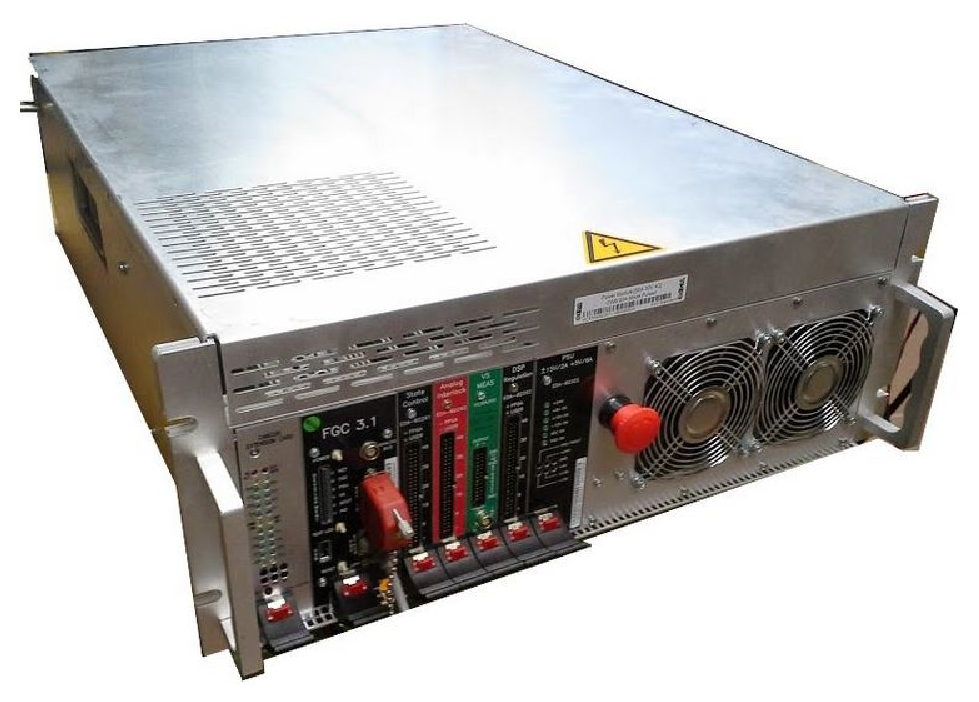
\includegraphics[width=0.8\columnwidth]{pics/housing_rack.eps}
\caption{CANCUN power converter. } 
%The FGC also collects and reports all statuses, faults, and measurements from various parts of the system and serves as the interface towards higher levels layers of the complex accelerator control architecture.}
\label{fig:cancun}
\end{figure}

\iffalse
\subsection{Track Delay and Tracking Error}
\label{track_error_definition}
%Before proceeding to the next section, it is imperative to first assert how the error is determined between the reference and the output current. 
In typical control applications, the error is usually calculated as the difference between the reference and the output sampled at a given time $t$. However, for some power converter control applications at CERN, the error is actually calculated as the difference between a delayed version of the reference input and the output at time $t$. 
The delayed reference input (for an arbitrary, positive delay) can be approximated as the output of the following interpolating filter:
\begin{equation}
\label{eq:del_filt}
\begin{aligned}
H(z^{-1})=z^{-\lfloor \tau \rfloor} \left(  1-(\tau - \lfloor \tau \rfloor) + (\tau - \lfloor \tau \rfloor)z^{-1}   \right) \\ \ \tau \in \mathbb{R}
\end{aligned}
\end{equation}
where $\tau$ is a (generally fractional) delay (expressed in units of the sampling time $T_s$), and the $\lfloor \cdot \rfloor$ operator represents the floor function which maps the real number in the argument to the largest integer not greater than that number. The use of (\ref{eq:del_filt}) allows one to interpolate the delayed reference signal between sampling points and calculate a more accurate error signal. For a given reference signal $\tilde{r}(z^{-1})$, the interpolated (causal) discrete-time reference signal will be
\begin{equation}
\label{eq:del_filt_new}
\begin{aligned}
r[n] &= \mathcal{Z}^{-1} \{ H(z^{-1}) \tilde{r}(z^{-1})\} \\
&=(1-\tau_{\text{frac}}) \tilde{r}[n-\lfloor \tau \rfloor]+ \tau_{\text{frac}} \tilde{r}[(n-1) -\lfloor \tau \rfloor]
\end{aligned}
\end{equation}
where $\tau_{\text{frac}} = \tau - \lfloor \tau \rfloor$ and $n \in \mathbb{Z}$. Therefore, for any discrete time instant $n$, the error is determined as $e[n] = r[n] - y[n]$, where $y[n]$ is the output response. For the purposes of this paper, $\tau$ is termed as the `track delay', and its value is related to the group delay of the closed-loop system:
\begin{equation}
\tau_g(\omega) = - \frac{d\phi_T(\omega)}{d\omega}; \quad \tau = \tau_g(0) \\
\label{eq:group_delay_theor}
\end{equation}
where $\phi_T(\omega)$ is the phase response associated with the closed-loop FRF.
%\end{remark}
\fi



\section{Case Study Results}
\label{sec:5}
This case study is devoted to the CANCUN power converter control system, as described in the previous section. The objective is to control the output current $i_D$ that is injected into the particle accelerator magnets in order to ensure proper particle trajectories. The profile of the reference current $i_R$ associated with the Q-STRIP magnet is shown in Fig.~\ref{fig:QCF_ref}.  For this application, the challenging task is to ensure the tracking performance; it is required that the error remains within $\pm 1000$ ppm\footnote{The calculation for obtaining the error in ppm is performed by taking the raw data for the error and scaling it by a factor of $\sfrac{10^6}{100}$. The factor of $100$ represents the nominal current ($100$ $A$) of the power converter for the Q-STRIP magnets.} during the fast transient and remains within $\pm 100$ ppm during steady state. The proposed controller design method was used to synthesize an $RST$ controller for this specific requirement. Experimental validation was performed by means of the test setup presented in \ref{test_setup}. 
\begin{figure}
\centering
\includegraphics[width=\columnwidth]{pics_prbs/reference.eps}
\caption{The reference current associated with the QCF circuit configuration. The blue-dashed line indicates the time when the error must remain within $\pm 1000$ ppm; the red-dashed line indicates the time when the error must remain within $\pm 100$ ppm;}
\label{fig:QCF_ref}
\end{figure}

The Q-STRIP magnet is represented as an $RL$ circuit, and the dynamics of this circuit are dominant over the other components of the system. Thus a first order model with delay (i.e., $G_m(s) = e^{-sT_d}(L_m s + R_m)^{-1}$, where $R_m$ is the circuit resistance, $L_m$ is the circuit inductance, and $T_d$ is the time delay) is appropriate to approximate the dynamics of the plant. For this case study, the model parameters are:
\begin{equation*}
R_m = 164.3 \: m \Omega; \quad L_m = 736.4 \: \mu H; \quad T_d = 275.4 \: \mu s
\end{equation*}
The model is then discretized using the zero-order-hold method and used to design an $RST$ controller based on the model-reference control (MRC) strategy \cite{LZ06}. In this particular implementation of the strategy, the transfer function between the reference signal and output depends on the location of the single zero (which comes from modeling the fractional delay) of the system \cite{KNM15}. According to \cite{LZ06}, if the fractional delay of the system is less than $0.5T_s$, then the zero of the system can be cancelled (which enables the tracking and regulation performances to be achieved without approximation). However, at CERN, this benchmark is modified such that the zero of the system is cancelled if the fractional delay is less than $0.4T_s$. In this case, the reference model is selected such that the transfer function from the reference input to the output will be a pure delay. However, if the fractional delay is greater than $0.4T_s$, then the corresponding zero cannot be cancelled, and the transfer function from the reference input to the output is represented as a fractional delay. The main difficulty of this approach is that the choice of the observer poles that lead to a good robustness margin is not trivial. The current practice at CERN is a trial-and-error approach to meet the control specifications. The main objective of this case study is to propose a systematic optimization based approach to compute the optimal controller parameters and guaranteeing robustness with respect to model uncertainties. 

For this type of application, it is a challenging task to achieve tracking and a good robustness margin simultaneously. With the MRC method, the auxilary  poles must be placed in an iterative fashion in order to achieve the desired modulus margin of $0.5$. However, the method proposed in this paper does not need a parametric identification or any iterative tuning scheme. It is a straightforward systematic design methodology that takes also into account the frequency-domain uncertainties, which increases the robustness of the design process.

\subsection{Frequency Response Function Measurement}
A pseudo-random binary sequence (PRBS) signal was used as the input voltage reference of the open-loop system in order to capture the dynamics of the process. The PRBS is a deterministic signal which has characteristics similar to that of white noise and is usually used for system identification. From Fig.~\ref{fig:ident_block}, the measurement process will capture the dynamics from the input of the DAC (with input voltage $v(t)$ representing the reference voltage of the voltage source) to the output of the DLPF (with output current $i(t)$ representing the measured current to be fed back to the $RST$ controller). 

Unfortunately, the FGC3 is limited by the amount of input samples that can be programmed to execute the PRBS signal (a maximum of $1023$). Therefore, to maximize the quality of the measurement, a PRBS signal of length $511$ ($9$-bits) with $2$ periods was injected as the input of the open-loop process. Note that a PRBS of length $1023$ ($10$-bits) with one period could also be used as the input; however, the output of such a reference will contain transients and must be considered as an aperiodic signal and thus increasing the truncation errors. 

A total of $5$ experiments were performed with the PRBS clock period $T_{cl} = 100 \: \mu s$; the acquired periods (with transients removed in post-processing) could then be merged together. For a signal of length $511$, the frequency resolution is limited to $255$ points. A DC gain was added to this measurement in order to increase the resolution at lower frequencies (due to the low resolution resulting from the PRBS identification). This DC value was determined by simply applying a DC voltage $v(t) = V_{dc} = 1V$ and obtaining the value $i(t) = I_{dc}$. With $95\%$ confidence, the uncertainty associated for this gain can be calculated as 
$$|W_n(e^{-j\omega_0})| = 2\sigma_I / \sqrt{N_s} = 3.51 \times10^{-4}$$ 
where $\omega_0$ is chosen to be arbitrarily small ($\omega_0 = 0.2\pi$), $N_s = 12000$ is the length of the signal, and $\sigma_I = 0.0192 \: A$ is the root-mean-square of the measurement noise. This specific value of the uncertainty is for the DC gain and not for all of the other corresponding frequencies. The uncertainties for the remaining frequencies were determined with (\ref{eq:uncertainty_radius}). The PRBS input signal along with the resulting output response are shown in Fig.~\ref{fig:PRBS}. 

\begin{figure}
\centering
\includegraphics[width=\columnwidth]{pics_prbs/prbs_time.eps}
\caption{PRBS signal used for the input voltage $v(t)$ of the open-loop system along with the resulting output current $i(t)$.}
\label{fig:PRBS}
\end{figure}
The FRF of the open-loop plant was then obtained as $G\jo=\mathcal{F}[i(t)]/ \mathcal{F}[v(t)]$ (where the operator $\mathcal{F}$ signifies the Fourier Transform). From (\ref{eq:uncertainty_radius}) and (\ref{eq:noise_spectrum}), the additive uncertainty associated with each frequency can be computed. Fig.~\ref{fig:plant_uncertain} displays a Bode diagram of $G\jo$ with the corresponding uncertainty bounds. 

\begin{figure}
\centering
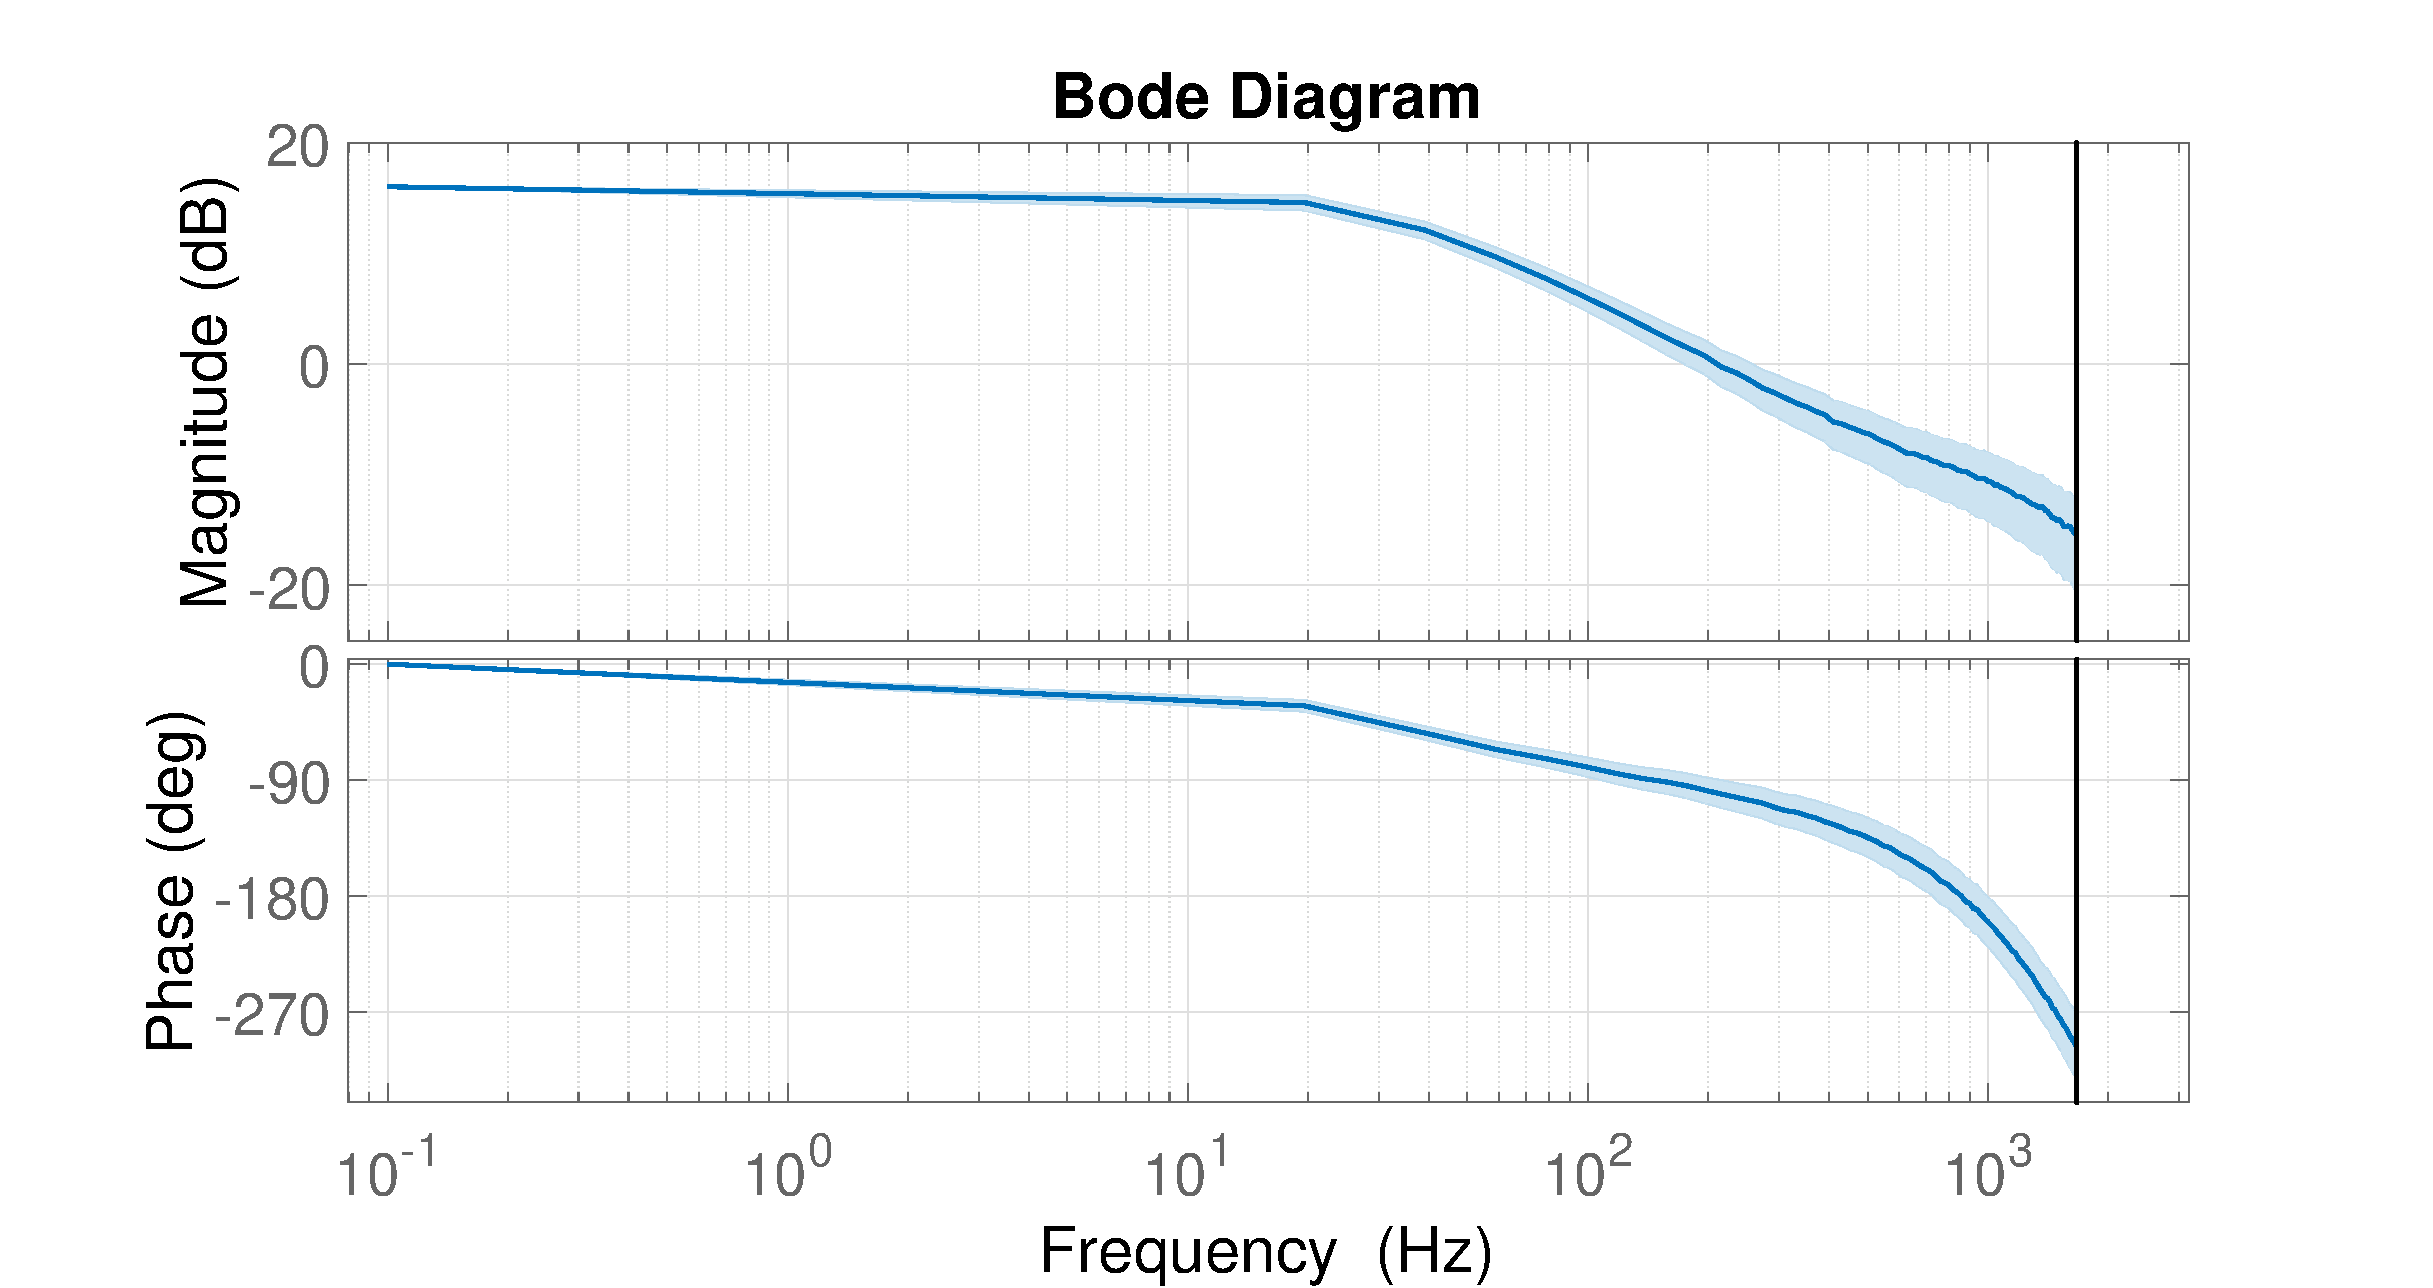
\includegraphics[width=\columnwidth]{pics_prbs/bode.eps}
\caption{Bode diagram of $G\jo$ with additive uncertainty bounds for the corresponding frequency points.}
\label{fig:plant_uncertain}
\end{figure}



%\begin{figure}[!b]
%\centering
%\resizebox{1\columnwidth}{!}{\input{pc_drawing_ident.eps_tex}}
%\caption{A block diagram which depicts the system structure and the identified process. Identified components (red-dashed blocks); unidentified components (blue blocks).}
%\label{fig:ident_block}
%\end{figure}

%\begin{lemma}
%Suppose that a bound is set such that $\| \mathcal{S}_0 \| ^{-1}_{\infty} > m_d$, where $m_d$ is the desired minimum value of the modulus margin. Then a condition for ensuring this constraint can be formulated as follows:
%\begin{equation}
%\begin{aligned}\label{eq:con_mm}
%m_d|MS(\rho)| < \mathcal{R}e\{\psi(\rho) \}& \\
%\forall \omega \in \Omega &
%\end{aligned}
%\end{equation}
%\end{lemma}
%
%\begin{IEEEproof}
%The proof for this condition is very similar to the proof of the constraint in Theorem 1. Here, the radius of the circle in Fig.\ref{fig:circle} is now $m_d|MS(\rho)|$ instead of $\gamma^{-1}|W_q \Delta_q(\rho)|$.
%\end{IEEEproof}
%Since the circle associated with this constraint is centered at $\psi(\rho)$, then the inclusion of this constraint with the $\mathcal{H}_{\infty}$ loop-shaping constraint still guarantees necessity and sufficiency of Theorem \ref{Th2}.
%
%

\subsection{Controller Stability}
\label{sec:con_stab}
Computation of an unstable controller should generally be avoided \cite{LZ06}. The logic behind this assertion has to do with the practical implications involved with a feedback control system.  Suppose that the plant $G(z^{-1}) = N(z^{-1})M^{-1}(z^{-1})$ is analytic outside the unit circle. For the $RST$ structure, it is evident that if the polynomial $S(z^{-1},\rho)$ possesses zeros outside the unit circle, then the open-loop system will become unstable (assuming no zero-pole cancellations occur with $R(z^{-1},\rho)$ and $S(z^{-1},\rho)$). In order to avoid this impairment, it is required to impose a constraint such that the polynomial $S(z^{-1},\rho)$ possesses zeroes inside the unit circle. This rationalization leads to the following lemma:

\begin{lemma}
Suppose that $S(z^{-1},\rho)$ is parameterized as in (\ref{eq:Sc}). Then a sufficient (convex) condition to ensure that the zeros of $S(z^{-1},\rho)$ remain inside the unit circle is
\begin{equation} \label{eq:con_con}
\Re \{S(\rho) \} > 0; \quad \forall \omega \in \Omega
\end{equation}
\end{lemma}
\begin{IEEEproof}
First note that a strictly positive real transfer function (and its inverse) is stable. $\Re \{S(\rho) \} > 0$ implies that the Nyquist diagram of $S(\rho)$ will not encircle the origin. Therefore, $S^{-1}(\rho)$ will not encircle the origin, and $S(\rho)$ is stable.    
\end{IEEEproof}


\subsection{Weighting Filter Design}
\label{sec:weighting_filter}
The $\mathcal{H}_{\infty}$ criterion in (\ref{eq:true_hinf}) is a very powerful design tool, as it provides the capability to shape any sensitivity function $\mathcal{S}_q$ based on the specifications set by a weighting filter. However, in certain design schemes at CERN, it may be desired to bound a sensitivity function to a particular value. For example, it may be desired to simply impose a lower-bound on the modulus margin in order to obtain the intended robust performance of a system. The modulus margin is defined as the minimum distance between the critical point $(-1+j0)$ and the Nyquist plot of the open loop transfer function, and can be expressed as
\begin{equation}
M_m = \| \mathcal{S}_1 \| ^{-1}_{\infty}
\end{equation}
In general, it is desired to obtain a minimum value of the modulus margin in order to ensure a sufficiently robust system. Let $m_d$ denote the minimum value of the desired modulus margin such that $M_m > m_d$. According to \cite{LZ06}, typical values for a good modulus margin are $M_m \geq 0.5 \ (-6 \; dB)$ (which ensures a gain margin of at least $6 \; dB$ and a phase margin of at least $29^{\circ}$). A constraint for ensuring a minimum value of the modulus margin can be constructed as follows:
\begin{equation}
  \| m_d \mathcal{S}_1 \|_\infty < 1 
\end{equation}
This constraint is a special case of the $\mathcal{H}_\infty$ constraints with $W_1(e^{-j\omega})=m_d$ and can be convexified using the results of Theorem \ref{Th2}.

For this particular case study, it is desired to obtain the best tracking performance (i.e., by minimizing $\gamma$ in $\|W_3 \mathcal{S}_3 \|_{\infty} < \gamma$) while ensuring reasonable stability margins. The weighting filter $W_3$ is chosen based on the fact that $\mathcal{S}_2^d + \mathcal{S}_3^d = 1$, where $\mathcal{S}_3^d$ is the desired error sensitivity function and $\mathcal{S}_2^d$ is the desired complementary sensitivity function (i.e., the closed-loop transfer function). $\mathcal{S}_2^d$ was chosen as a standard second order transfer function  with the given form:
\begin{equation}
\mathcal{S}_2^d(s) = \frac{\omega_d^2}{s^2 + 2\zeta \omega_d s + \omega_d^2}
\end{equation}
where $\zeta$ is the damping factor and
\begin{equation*}
\omega_d = \frac{2 \pi f_d}{\sqrt{1-2\zeta^2 + \sqrt{2-4\zeta^2 + 4\zeta^4}}}
\end{equation*}
where $f_d$ is the desired closed-loop bandwidth. Note that it is possible to consider a continuous-time transfer function for this specification since the proposed method implements a frequency-domain approach. Since $\mathcal{S}_2^d = 1- \mathcal{S}_3^d$, an appropriate filter for the error sensitivity function can be devised as
\begin{equation}
W_3(s) = \frac{s^2 + 2\zeta \omega_d s + \omega_d^2}{s(s+2\zeta \omega_d)}
\end{equation}
Due to the fact that $W_3(j\omega_k)$ is evaluated at a finite number of frequency points with $\omega_0 \neq 0$, then the integrator in $W_3$ does not pose problems with boundedness.

%For discrete-time systems, there are limitations with regards to the achievable closed-loop bandwidth of a system. According to \cite{LZ06}, the achievable closed-loop bandwidth is bounded by the following constraint:
%\begin{equation} \label{eq:bandwidth}
%f_s \in [6,25]f_d
%\end{equation}
A simulation was performed to determine the bandwidth that is required in order to satisfy the desired error specifications. At CERN, the error is calculated with respect to a delayed reference input (i.e., $e(t) = r(t-\tau) - y(t)$). By assuming that the closed-loop response behaves as $\mathcal{S}_2^d$, the bandwidth $f_d$ can be selected such that the error between the delayed reference input and output is within $\pm 100$ ppm. For this second order response, this delay was analytically derived as $\tau = 2\zeta/ \omega_d$. It was determined that $f_d = 300 \ Hz$ with $\zeta = 0.8$ satisfies these requirements. 
%Since the sampling frequency for the power converter control system is $3.333 \; kHz$, then $f_s/f_d$ satisfies the constraint in (\ref{eq:bandwidth}). 


\subsection{$RST$ Controller Synthesis}
\label{synthesis}
The voltage applied to the magnet by the voltage source and the relative current are both sampled at 10  kHz while the control loop is run $3$ times slower (i.e., $f_s = 3.333$ kHz and $T_s = 300 \  \mu$s, where $f_s$ and $T_s$ are denoted as the sampling frequency and sampling time of the control loop, respectively).  Since the plant is stable, then a possible selection for the coprime factors is $N\jo = G\jo$ and $M\jo = 1$. For proper implementation within the proprietary power converter control software, it is required that all the open-loop poles remain on or within the unit circle, i.e. the controller should be marginally stable. This implies that the zeroes of $S(\rho)$ must lie on or within the unit circle. Since the reference current is close to a ramp signal, to achieve adequate performance, $S(z^{-1},\rho)$ must incorporate a double integrator: $S(z^{-1},\rho) = (1-z^{-1})^2S^\star(z^{-1},\rho)$. With the FRF measured by means of the PRBS excitation, the constraints for the convex optimization problem are formulated. With a minimum value of $m_d=0.5$ set for the modulus margin, the following optimization problem must be solved: 
\begin{equation} \label{eq:min_sim}
\begin{aligned}
& \underset{ \rho \in \mathbb{R}}{\text{minimize}}
& & \gamma  \\
& \text{subject to:} & & \Re\{\psi \jrok \} > x_r \jrok  \\
& & & \Re\{\psi \jrok \} > m_d|S \jrok|  \\
& & & \Re \{S^{\star}\jrok \}  > 0 \\
& & & \mbox{for }k = 0,\ldots,\eta
\end{aligned}
\end{equation}
where 
\begin{equation*}
\psi \jrok = S \jrok  + N\jok R \jrok  
\end{equation*}
and $x_r \jrok$ is defined as in (\ref{eq:rad_robust_design}). The first inequality in (\ref{eq:min_sim}) ensures that $\mathcal{H}_{\infty}$ nominal performance is achieved for the $RST$ structure whilst considering the frequency dependent uncertainties. The second inequality ensures that the modulus margin is at least $0.5$. With the additional low-frequency measurement at $\omega_0$,  there will be a total of $256$ frequency points ($\eta = 255$, $\omega_k \in (0,\pi f_s] \ \forall k$).


\subsection{Optimization Results} 
\label{sec:opt_results}
The SDPT3 open-source optimization package was used in conjunction with Matlab to perform the bisection algorithm \cite{SDPT3}. The solution to the optimization problem in (\ref{eq:min_sim}) leads to a 9-th order stable controller that achieves the desired performance. The main parameters of the bisection algorithm are tabulated in Table.~{\ref{tab:gamma}. 
%Note that the orders of $R$ and $T$ are chosen to be equal. Their orders are larger than $S$ to ensure better tracking performance. All the zeros of $S^{\star}(z^{-1})$ lie inside the unit circle, and thus ensuring that the open-loop system remains marginally stable. 


\begin{table}
\centering
\caption{Parameters resulting from the bisection algorithm.}
\label{tab:gamma}
\begin{tabular}{c|cc}
\textit{\textbf{Parameter}} & \textit{\textbf{Value}} & \textit{\textbf{Unit}} \\ \hline
$\gamma_{\max}$              & $2.5$                    & -                      \\
$\gamma_{\min}$              & $0$              & -                      \\
$\gamma_{\text{tol}}$              & $10^{-6}$               & -                      \\
$\gamma_{\text{opt}}$              & $1.202$                & -                      \\
\textit{Optimization time}\footnotemark  & $61.3$                 & $s$                   
\end{tabular}
\end{table}
\footnotetext{This optimization time was calculated based on a computer having the following hardware specifications: Intel-Core i7, 3.4 GHz CPU, 8 GB RAM. The optimization algorithm was run using MATLAB version 8.6.0.267246 (R2015b) on a Windows 7 platform (64-bit).}

%The FRF for the desired and actualized closed-loop response is shown in Fig.~{\ref{fig:cl_freq}. 
%The expected closed-loop bandwidth is approximately equal to the bandwidth chosen for the desired specifications (i.e., $170 \: Hz$). 
The obtained output sensitivity function $| \mathcal{S}_1|$ is depicted in Fig.~{\ref{fig:sens_freq}}. It can be observed that this sensitivity function is indeed bounded by the modulus margin constraint and that a modulus margin of $0.5$ is obtained. %The calculated gain and phase margins are  $11.1 \ dB$ and $66.2^{\circ}$, respectively. 

%\begin{figure}
%\centering
%\includegraphics[width=\columnwidth]{pics_prbs/closed_loop.eps}
%\caption{Comparison between the FRF's of the desired and expected closed-loop response. FRF of the desired closed-loop transfer function $\mathcal{T}_d(s)$ (solid-green line); FRF of the actual closed-loop response (solid-blue line). }
%\label{fig:cl_freq}
%\end{figure}

\begin{figure}
\centering
\includegraphics[width=\columnwidth]{pics_prbs/sens_S0.eps}
\caption{FRF of the output sensitivity function $\mathcal{S}_1$ (solid-blue line) and the bound for the modulus margin.}
\label{fig:sens_freq}
\end{figure}

For the reference current applied to this system, the error between the reference and the output current is determined by shifting the reference current such that a minimum peak error is achieved; this will be shown in the next section.
%A plot of the group delay (in units of $T_s$) is shown in Fig.~\ref{fig:track_delay}. 
%For the reference current applied to this system, the track delay $\tau$ can be estimated as the DC value of the group delay (given by (\ref{eq:group_delay_theor})) , which is approximately $829.9 \: \mu s$ (or $\tau = 2.766$ $T_s$). The reference current is delayed by using (\ref{eq:del_filt_new}) in order to calculate the experimental error (which is shown in the next section).

%\begin{figure}
%\centering
%\includegraphics[width=\columnwidth]{pics_prbs/group_delay.eps}
%\caption{A frequency-domain plot of the calculated group delay (in units of the control loop sampling time $T_s$). For the current reference profile, the estimated delay (used for calculating the error) is the DC value of the group delay; this DC value is approximately equal to $10.126 \: [T_s]$.}
%\label{fig:track_delay}
%\end{figure}

%\subsection{Experimental Validation - Frequency Domain}
%The frequency response of the closed-loop system was measured by means of a dedicated experiment. The converter was programmed to produce sinusoidal currents at given frequencies with small amplitudes ($0.4 \: A_{peak}$); both the reference and measured current were recorded with custom software diagnostic tools. The amplitude and phase of both currents were estimated by means of a three-parameter sinefit \cite{1057}, \cite{MLM12}.  
%The main features of the diagnostics tools used for signal acquisition are: 
%\begin{itemize}
	%\item sampling frequency of $10 \: kHz$
	%\item record length of $1.2 \: s$ irrespective of the frequency being probed
%\end{itemize}
%These features posed several limitations on the frequency range that could be probed:
%\begin{itemize}
	%\item \emph{high frequencies} are limited to $1$ $kHz$ by the need of having enough samples per period to properly estimate the amplitude and phase (at $1$ $kHz$, only $10000/1000 = 10$ samples are acquired for each period; furthermore, the first harmonics of $50$ $Hz$ have been discarded for this measurement in order to avoid residual ripple)  
	%\item \emph{low frequencies} are limited to about $1 \: Hz$ by the need of acquiring at least $1$ period to properly estimate both amplitude and phase
%\end{itemize}
%
%The closed-loop frequency response and the group delay (numerically calculated from the measured phase by means of (\ref{eq:group_delay_theor})) are shown in Fig.~\ref{fig:closed_loop_meas} and Fig.~\ref{fig:group_delay_meas}, respectively. From Fig.~\ref{fig:closed_loop_meas}, it can be observed that the actual closed-loop frequency response closely matches that of the desired response. Additionally, the experimental error obtained from the average value of the measured group delay and the value obtained from the DC value of the group delay in the previous section ($\tau_g(0) = 1.0126 \: ms$) is only $0.85 \: \%$.
%
%\begin{figure}
%\centering
%\includegraphics[width=\columnwidth]{pics_prbs/Experimental_Bode.eps}
%\caption{Measured frequency response of the closed-loop system (solid-blue) and the desired closed-loop system (solid-red).}
%\label{fig:closed_loop_meas}
%\end{figure}
%
%\begin{figure}
%\centering
%\includegraphics[width=\columnwidth]{pics_prbs/Experimental_Group_Delay.eps}
%\caption{The measured group delay (solid-blue) along with the group delay calculated from $\mathcal{T}_d$ (solid-red). The track delay is estimated as the average value of the data points shown in solid-black. This value is determined to be $1.042 \: ms$.}
%\label{fig:group_delay_meas}
%\end{figure}

\subsection{Experimental Validation and Comparison}
The reference and measured currents were acquired for the profile required by a specific Q-STRIP magnet (Fig.~\ref{fig:QCF_ref}). As stated in section \ref{sec:weighting_filter}, the error is calculated with respect to a delayed reference input (i.e., $e(t) = r(t-\tau) - y(t)$). For comparison purposes,  the value of $\tau$ was found by shifting the reference profile such that the minimum peak error was achieved. A total of $10$ experiments were performed; the error for both the model-based and data-driven based designs (with the associated error-bars showing the minimum and maximum errors at each sampling instant) are shown in Fig.~\ref{fig:error}. It can be observed that both designs are comfortably within the $\pm 1000$ ppm fast-transient requirement and within the $\pm 100$ ppm steady-state requirement. Indeed, both controllers achieve $\pm 100$ ppm even during the fast-transients. However, the proposed method ensures that all of the design requirements are met while eliminating the iterative process of attaining robust performance from the model-based methodology. Therefore, the proposed data-driven method proves to be superior as it achieves all of the design objectives in a single attempt. 

%\begin{figure}
%\centering
%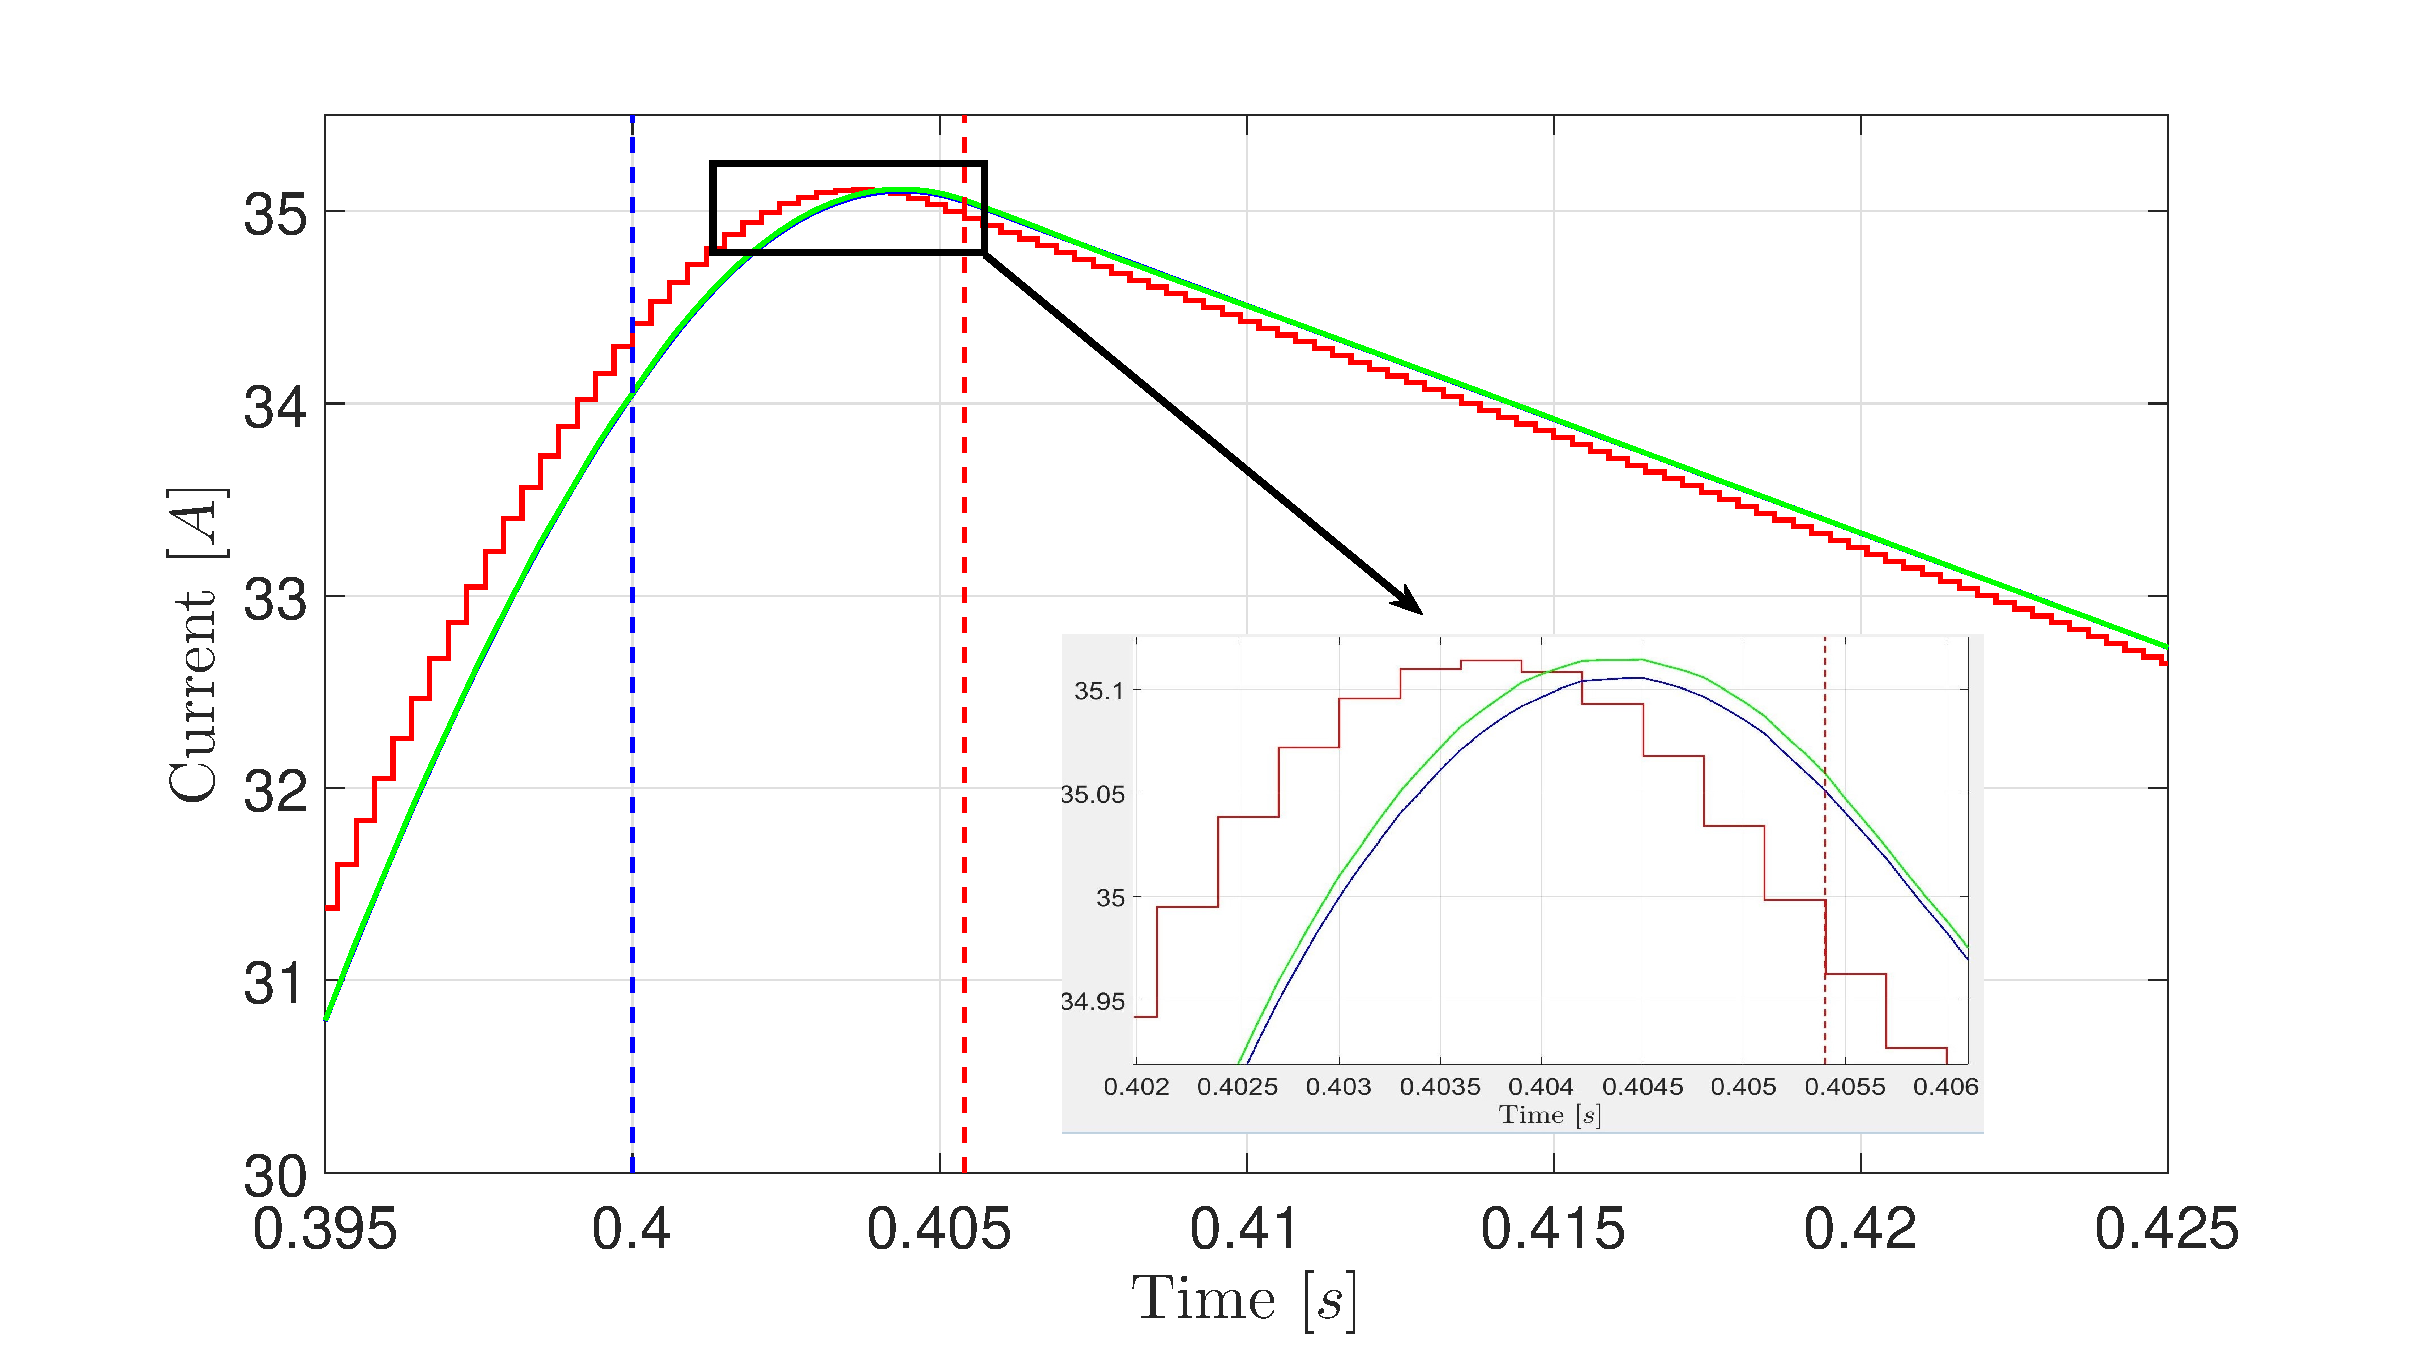
\includegraphics[width=\columnwidth]{pics_prbs/time_comp_2.eps}
%\caption{Comparison between the reference current (solid-red line), the output current resulting from the model-based controller (solid-blue line) and the output current resulting with the proposed method (solid-green line). The accelerator beam is applied at the time indicated with the dashed-blue line ($0.4s$); the error must be calculated after this time. The error after the time indicated with the dashed-red line ($0.4054s$) must be within $\pm 100$ ppm.}
%\label{fig:output}
%\end{figure}

\begin{figure}
\centering
\includegraphics[width=\columnwidth]{pics_prbs/error_comp_shift.eps}
\caption{Comparison between the error resulting from the model-based design (solid-black line with red error-bars) and the error resulting with the proposed method (solid-black line with green error-bars). %The accelerator beam is applied at the time indicated with the dashed-blue line ($0.4s$); the error must be calculated after this time. The error after the time indicated with the dashed-red line ($0.4054s$) must be within $\pm 100$ ppm.}
}
\label{fig:error}
\end{figure}



\section{Conclusion}
\label{sec:6}
A new data-driven method for computing a robust controller that attains $\mathcal{H}_{\infty}$ performance has been presented. A frequency-domain approach has been used in order to avoid the problem of unmodeled dynamics associated with parametric models. The necessary and sufficient conditions for the existence of $RST$ controllers with multiple $\mathcal{H}_\infty$ performance have been developed in terms of a set of convex constraints.  Constraints have been devised in order to design a controller which considers frequency dependent uncertainties, ensures a minimum value for the modulus margin, and to assure the controller stability. This method has been applied to a power converter control system which uses an $RST$ controller structure and is used for experimental purposes at CERN. In the case study presented in this paper, it has been shown that the proposed data-driven method offers an optimization-based systematic approach that leads to low-order $RST$ controllers meeting the challenging specification for particle trajectory tracking. With the proposed methodology, the process of obtaining a model and iteratively tuning the desired closed-loop bandwidth to attain the proper stability margins is eliminated whilst achieving the desired tracking performance. 

%For further research, it will be desired to determine the order of the controller polynomials that will produce the optimal tracking performance while attaining adequate disturbance rejection. 

%This paper has proposed a new method for computing multivariable SP controllers with $H_\infty$ performance. The method is based on a convex approximation of the $H_\infty$ robust performance criterion in the Nyquist diagram. This approximation relies on the choice of a desired open-loop transfer function $\vec{L}_D$ for the dead-time free model of the plant. With a linearly parameterized controller, one possesses the flexibility to design PI, PID, or higher order controllers for a system. For the industrial processes considered in this paper, the proposed method has been proven to be robust; $H_{\infty}$ performance was achieved for MIMO systems with both multiplicative and time delay uncertainties. Moreover, the solution to the optimization problem generates a controller such that a system becomes decoupled and simultaneously optimizes the single-loop performances of the SISO subsystems.

%\appendix[]
%\begin{table}[H]
%\centering
%\caption{Solution to the optimization problem in (\ref{eq:min_sim}); parameters reported with a reduced number of significant digits.}
%\label{my-label}
%\begin{tabular}{c|c|c}
%$\rho_R$ & $\rho_S^{\star}$ & $\rho_T$ \\ \hline
%$2.064$      & $1$              & $0.9025$      \\ \hline
%$- 0.9093$      & $- 0.4093$              & $- 0.3494$      \\ \hline
%$- 1.08$      & $- 1.014 $              & $- 0.004285$      \\ \hline
%$0.4282$      & $0.05461$              & $- 0.335$      \\ \hline
%$- 1.152$      & $- 0.08757$              & $0.01702$      \\ \hline
%$0.5985$      & $0.1138$              & $- 0.1231$      \\ \hline
%$0.06517$      & $0.3425$              & $0.08679$     \\ \hline
%$0.1158$   &       -       & $- 0.06379$     
%\end{tabular}
%\end{table}

\iffalse
\section*{Acknowledgement}
The authors of this paper would like to thank Louis de Mallac for his contribution to the experimental setup of the power converter control system and Quentin King (both with the TE department at CERN) for providing support for the controller implementation within the FGC software environment.
\fi


%\begin{IEEEbiographynophoto}
%Author1 Biography
%\end{IEEEbiographynophoto}
%\smallskip{}
%\begin{IEEEbiographynophoto}
%Author2 Biography
%\end{IEEEbiographynophoto}

%\bibliography{/Users/anicolet/Google Drive/EPFL Research/Publications/linear}
\bibliography{linear}

\iffalse
\vspace*{-2\baselineskip}

\begin{IEEEbiography}[{
\includegraphics[width=1in,height=1.25in,clip,keepaspectratio]{pics/bib_achille.eps}}]{Achille Nicoletti} was born in Quebec, Canada on June 20, 1983. He received both his B.Sc. in Physics and B.E.E degrees at Cleveland State University (USA) in 2011 (summa cum laude). He also received his M.Sc. in Electrical Engineering at the same university in 2012. During his studies in receiving his M.Sc. degree, he was recruited by Philips in Highland Heights, Ohio, where he was employed as an Electrical Design Engineer (II) and was responsible for designing the control system for the next generation computed tomography (CT) products. During this time at Philips, he received his Six Sigma Green Belt certification. In 2014, he decided to pursue a PhD in the field of control systems at the Swiss Federal Institute of Technology in Lausanne (EPFL), Switzerland. In the same year, he had been accepted to a doctoral fellowship program at CERN. His main research interests include robust data-driven control methods (frequency domain), and optimization in systems and control.
\end{IEEEbiography}

\vspace*{-2\baselineskip}

\begin{IEEEbiography}[{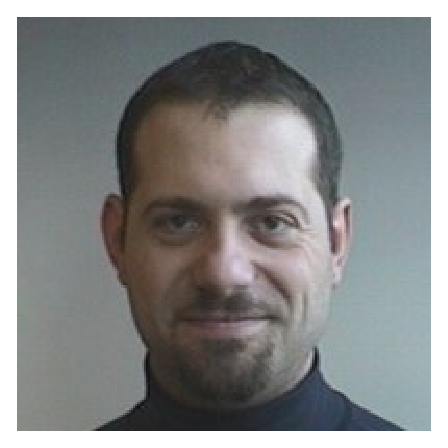
\includegraphics[width=1in,height=1.25in,clip,keepaspectratio]{pics/bib_michele.eps}}]{Michele Martino}
was born in Napoli, Italy, on July 23, 1975. He received the M.Sc. in Electronics Engineering (magna cum laude) and the Ph.D. in Electrical Engineering at the University of Napoli Federico II. PhD research was carried out at CERN on the high precision position survey of the Large Hadron Collider collimators. In 2004 he was with FIAT as control algorithm designer on Traction Control and then, in 2005, he joined I.N.F.N (Italian National Institute of Nuclear Physics) as fellow to work on the LHCb muon detector front end electronics test. Since June 2006 he is at CERN and in 2010 joined the Electrical Power Converter group to work on the high precision measurement and control of the power converters of CERN accelerators. His main research subjects are LVDT sensors characterization, high precision pulsed current and voltage measurements, digital control for power converters.
\end{IEEEbiography}

\vspace*{-2\baselineskip}

\begin{IEEEbiography}[{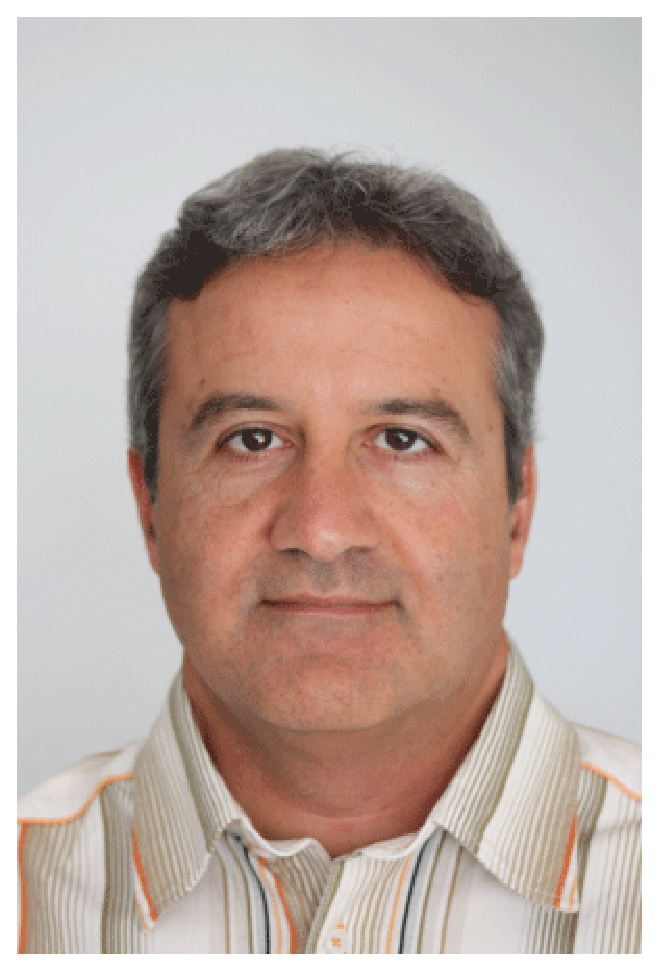
\includegraphics[width=1in,height=1.25in,clip,keepaspectratio]{pics/bib_alireza.eps}}]{Alireza Karimi} received his B. Sc. and M. Sc. degrees in Electrical Engineering in 1987 and 1990 from Amir Kabir University (Tehran Polytechnic). After 3 years of industrial experience he joined Institut National Polytechnique de Grenoble (INPG) in France and received his DEA and Ph. D. degrees both on Automatic Control in 1994 and 1997, respectively. He was Assistant Professor at Electrical Engineering Department of Sharif University of Technology in Teheran from 1998 to 2000. He is currently Senior Scientist at the Automatic Laboratory of Swiss Federal Institute of Technology in Lausanne (EPFL), Switzerland. He was an Associate Editor of European Journal of Control from 2004 to 2013. His research interests include closed-loop identification, data-driven controller tuning approaches and robust control.
\end{IEEEbiography}
\fi
\end{document}
